% Vorlage für ein Inforz
% Erstellt von: Tobias Otterbein, totterbein@d120.de, Stand: 31.08.2014
% Überarbeitet von Johannes Alef, jalef@d120.de, Stand 23.09.2014
% Darf beliebig für ein Inforz angepasst werden.
\documentclass[a5paper,pagesize,twoside,fontsize=8pt,DIV=15]{scrreprt}
\usepackage[a5paper, left=15mm,right=15mm,top=15mm,bottom=20mm]{geometry}
\usepackage[utf8]{inputenc}
\usepackage{inforz}
\graphicspath{{../shared/grafik}}


\usepackage{color}
\usepackage{contour}


% Sprache hier einstellen
\usepackage[english]{babel}

% Auskommentieren, wenn keine Links im Inhalt benötigt werden. 4. Option sorgt für 2-seitige PDF-Ansicht
\PassOptionsToPackage{hyphens}{url}
\usepackage[colorlinks=true,linkcolor=black,urlcolor=black,pdfpagelayout=TwoColumnRight]{hyperref}

\begin{document}

% Titelseite
\begin{titlepage}~
	%\ThisCenterWallPaper{1}{../grafik/oinforz_cover_ss20}


	%\begin{textblock*}{12cm}(4cm,7cm)
	%
\includegraphics[height=10.5cm]{../grafik/wesen/wesen_portal}
	%\end{textblock*}



	\begin{textblock*}{12cm}(4.5cm,1cm)
		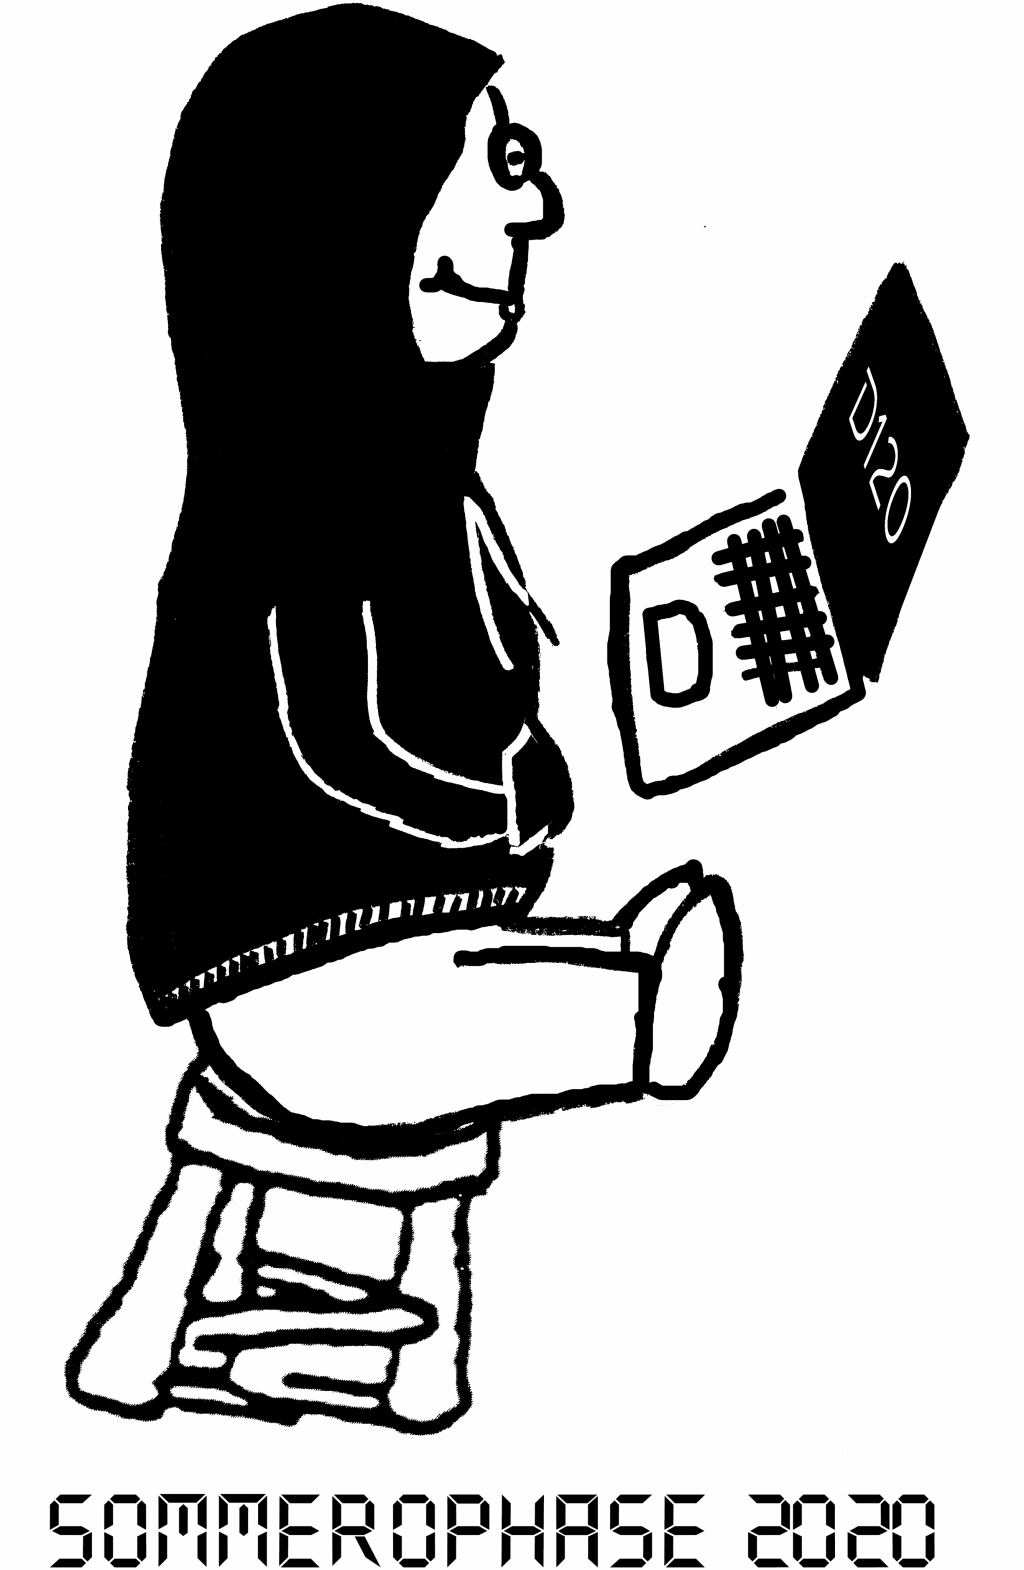
\includegraphics[width=2cm]{../grafik/wesen/wesen_ophase}
	\end{textblock*}

	\begin{textblock*}{12cm}(1.5cm,1cm)
		
\includegraphics[width=12cm]{../grafik/inforz_schwarz}
	\end{textblock*}


	\definecolor{mycolor}{HTML}{028902}  % diese Farben wurden willkürlich gewählt

	\begin{textblock*}{12cm}(6.5cm,4cm)
		\centering\fontsize{80}{25}\sffamily\textbf{
			\textcolor{mycolor}{Master } \\
			\textcolor{mycolor}{English}}
	\end{textblock*}


	\begin{textblock*}{12cm}(1.5cm,19cm)
		\centering\huge\sffamily\textbf{
			%\textcolor{black}{Welcome to the \ophase} \\
			%\textcolor{black}{by Fachschaft Informatik!} \\
		}
	\end{textblock*}


	\begin{textblock*}{7cm}(7cm,5.5cm)
		\begin{flushright}
			\large\sffamily\textbf{
				\textcolor{black}{Journal of students}\\
				\textcolor{black}{of computer science\\at the TU Darmstadt}}
		\end{flushright}
	\end{textblock*}

	\begin{textblock*}{18cm}(1.5cm,8cm)
		
\includegraphics[width=12cm]{../grafik/oinforz_cover_ss20}
	\end{textblock*}

	\begin{textblock*}{5cm}(1cm,9cm)
		\begin{rotate}{90}
			\sffamily\huge\textbf{
				\textcolor{black}{Inforz for \ophase}}
		\end{rotate}
	\end{textblock*}


	\begin{textblock*}{2cm}(1cm,14cm)
		\begin{rotate}{90}
			\sffamily\small \textcolor{black}{Price: invaluable}
		\end{rotate}
	\end{textblock*}


	\begin{textblock*}{2cm}(1cm,20cm)
		\begin{rotate}{90}
			\sffamily \textcolor{black}{ISSN: 1614-4295}
		\end{rotate}
	\end{textblock*}

\end{titlepage}
\newpage


% Stundenplan
\thispagestyle{empty}

\begin{figure}
    \centering
    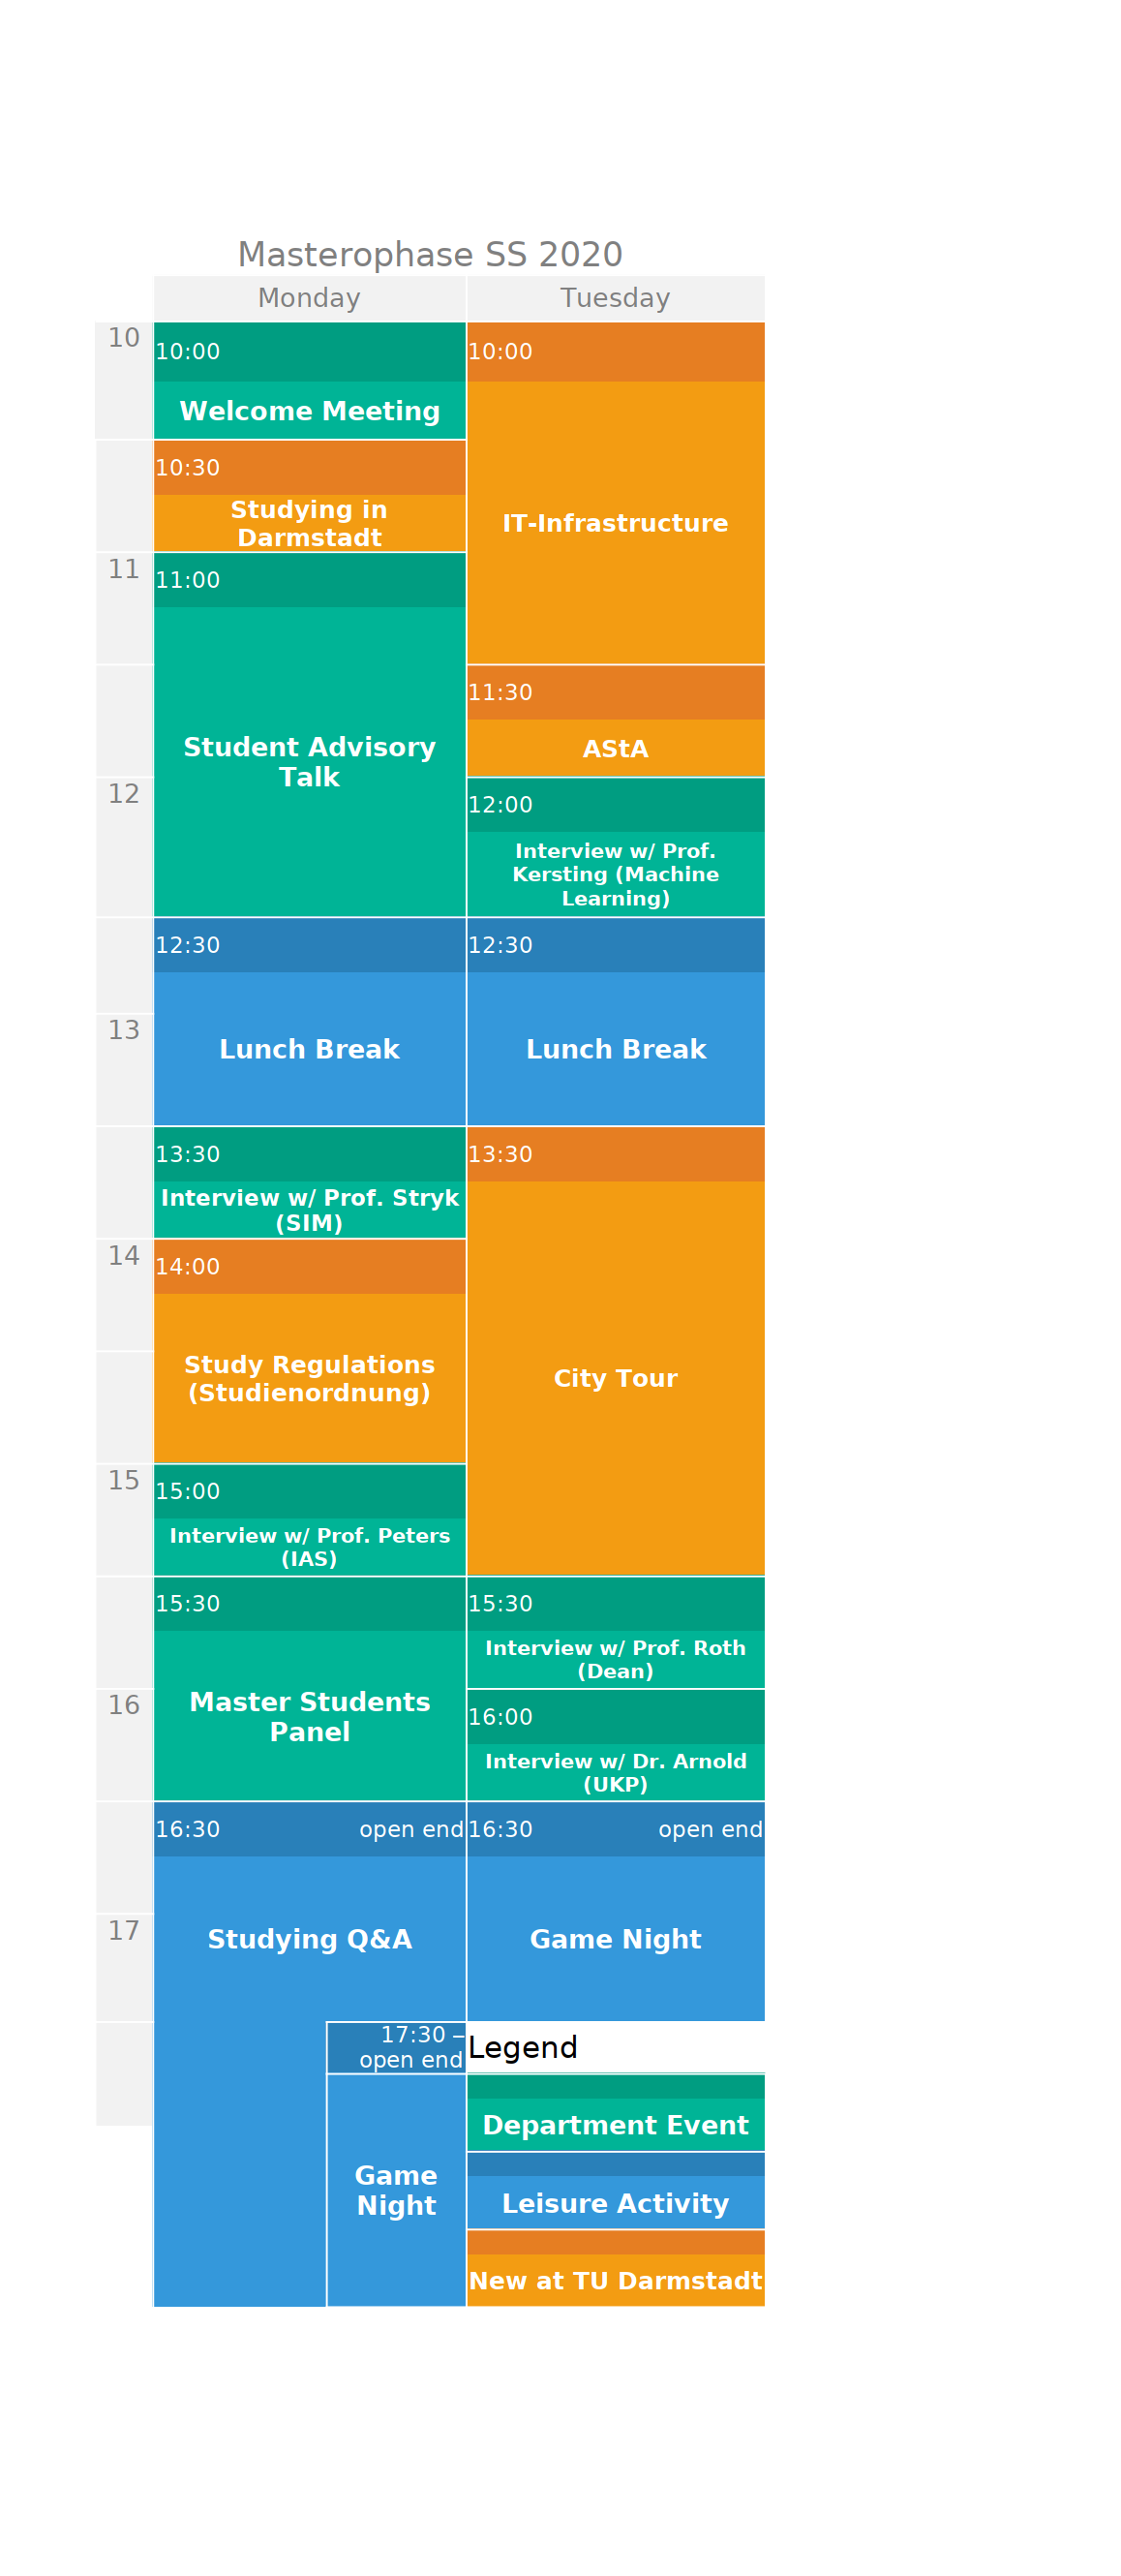
\includegraphics[angle=0,width=.8\linewidth]{stundenplan_cyberphase_de}
    \caption{Stundenplan der Cyberphase}
\end{figure}

\cleardoublepage



% Inhaltsverzeichnis
\tableofcontents

% Inhalt
\kapitel{Welcome}{../grafik/wesen/wesen_ophase}{}{}

\artikel{Foreword by the Department Chair and Dean of Studies}{Dear Students,}{

    We would like to welcome you most cordially to the Department of
    Computer Science of Technische Universit\"at Darmstadt.

    \

    We are very happy that you have chosen our department to continue your studies and we believe that you have made an excellent decision.
    Our CS department has been one of the first three Computer Science departments in Germany and it is also one of the most forward looking.
    We were one of the first departments to offer studies according to the new international Bachelor/Master system and for several years we have been offering the Master in Distributed Software Systems taught completely in English.
    However, the most important aspect for you is the quality of the education we offer.
    Based on a poll among human-resources managers at German companies, the Computer Science education in Darmstadt has been consistently ranked among the best at German universities.
    \

    %\bildmitunterschrift{../grafik/willkommen/muehlhaeuser_sw}{width=35mm}{Prof. Dr. rer. nat. Max Mühlhäuser}{}
    %\vspace{2mm}

    You come here with high expectations about how your learning experience will look like and we want to prepare you for what lies ahead.
    Success in your studies demand commitment, discipline, and adjusting to new ways of learning.
    You are used to studying hard and you already possess a solid foundation, but at the Master's level you will encounter courses that will introduce you to the state of art in their respective areas.
    We will challenge your analytic skills and your abilities for abstraction, as well as your aptitude for design and implementation of complex software.
    You must be able to work independently and proactively but also as part of a team.

    %\bildmitunterschrift{../grafik/willkommen/goesele_studiendekan}{width=35mm}{Prof. Dr.-Ing. Michael Goesele}{}
    %\vspace{2mm}

    Many of us in the faculty have studied abroad, so we know firsthand that it may take a few months to adjust to studying and living in a country with a different culture, life style, language, and more.
    Even the way the university and the study programs are organized may differ quite a bit from what you are used to.
    At the same time, many of us know how much of an enriching experience studying abroad is.
    Therefore, we highly encourage you to make the best of your time and take advantage of the many wonderful possibilities at and around TU Darmstadt.

    \

    To get you started, here are a few important tips to keep in mind:
    \\ \\
    \begin{description}
        \item[\parbox{\textwidth}{Be focused in your studies, but not over- \\
        ambitious.}]
            In the first term we recommend choosing courses that you are really interested in and whose content you can judge.
            Please, don't try to take too many courses at once: rather, focus on a few and do your best.
            It is important to start successfully and avoid being involved in too many activities.
        \item[Don't hesitate to ask for help.]
            If you have questions about organizational issues (e.g., you failed to register or de-register for an exam), if you have personal problems, or if you have problems with your visa, don't hesitate to ask for help.
            For study-related issues, in particular, the Examination Office and the Student Advisory Service are first points of contact.
            For all non-academic questions and issues, the International Student Service (ISS) is your best partner.
        \item[Be mindful of your visa status.]
            Please make sure that your visa status or resident permit in Germany remains always valid.
            It is important to remember deadlines and appointments with the authorities such as the Foreigners Office.
            Please pay close attention to any communication from the authorities -- keep your address current and carefully study your any letters in the mail.
        \item[Don't neglect the social side.]
            Skype \& Co.\ keep you in touch with home, but it is important to have a social life here.
            This is a great opportunity to make new friends and to learn about new things.
            The university offers a lot of social activities in which you can participate: sports, games, music, crafts, etc.
            And why not help out in the ``Fachschaft'', the representatives of the students, who put together this brochure?
        \item[Learn a few words of German.]
            German is a difficult language and no one expects you to master it in the two years you spend here.
            Having said that, knowing a few words of German will go a long way in your everyday life, be it in a restaurant, in a shop, or on the street.
            Just seeing that you make an effort can make a big difference, even if the conversation switches to English after a few sentences.
    \end{description}

    We, the Chair and the Dean for Studies of the Department of Computer Science at TU Darmstadt wish you a successful, exciting, educational, and happy time here in Darmstadt.
    We hope that you will enjoy your studies and that some time in the future you will look back fondly at the time you spent with us.

}{Prof.~Stefan Roth, Ph.D.~(Department Chair)\\ Prof.~Dr. rer. nat.~Michael Waidner (Dean of Studies)}

\vfill
\bildmitunterschrift{../grafik/comics/just_a_browser}{width=8cm}{}{xkcd.org}
\bildmitunterschrift{../grafik/comics/cautionary}{width=\textwidth}{}{xkcd.org}
\newpage

\artikel{Welcome to TU Darmstadt}
{The Fachschaft Informatik welcomes you to your studies at TU Darmstadt.}{
By now, you will probably have read and heard it several times already, but we, the Fachschaft Informatik\footnote{What -- or rather who -- we are and what we do, is described in the Article \textit{Questions and answers regarding the Fachschaft} on page~\pageref{FSarticle}}, would nonetheless like to heartily welcome you as well: to your master's degree studies, to Technische Universität Darmstadt, to Germany, and to a new chapter of your life in general!

You may have already encountered a number of things in and about Germany that may feel strange, foreign or simply new to you.
German culture is potentially very different from your own, and the university's as well as your study programme's structures are likely to be, too.
Do not despair, though, for you are neither the first nor the only one struggling with these changes.
Since many other students from abroad have been facing these same challenges in recent years already, the university and the computer science department have installed plenty of helpful facilities supposed to aid you with acclimatising to your master's degree programme.
One of those facilities is the orientation phase, or Ophase, which you are currently (or possibly soon) attending and which aims to provide you with all the knowledge needed to start your studies successfully.
In addition, there will be mentors (experienced students from the same programme as yours) to help you throughout your first semester who may also offer advise on other issues you may be facing in this country.
Last but not least, there is us, the Fachschaft Informatik (or \textit{student council}), a bunch of active volunteers who are always eager to help out all computer science students with advice concerning affairs related to the department or the various study programmes here.

It is our hope that during your studies you'll find new friends among your fellow students and that you may also find some time to expand your knowledge beyond this field of study alone.
After all, your studies here mark the beginning of a new episode of your life in which you have the chance to get to know a new country and to experience a whole different culture.
As such, we wish you all the best for your time here.
}
{Fachschaft Informatik}

%\vfill
\noindent
\bildmitunterschrift{../grafik/willkommen/fsbild}{width=.9\textwidth}{Some members of the \textit{Fachschaft} during winter term 2019/2020}{Tim Pollandt und Stefanie Blümer}

%\newpage

\artikel{Welcome to the Ophase}
{As you are holding this booklet in your hands and are reading this article, chances are that your orientation phase (or Ophase, in short) has just begun or you are right in the middle of it.}
{
    The orientation phase at the department of computer science sports a long history: it has existed for almost as long as the department of computer science itself has by now.
    Its aim is for you to get to know the university, especially the department of computer science, and to help you connect with your future fellow students.

    Every part of this event is organized and made possible by student volunteers eager to help new students like you to start their studies well prepared.
    The tutors taking care of you throughout the Ophase are students like you, who have also participated in an orientation phase in the beginning of their studies, and a few semesters later decided to pass on their experiences.

    This booklet, the Ophasen-Inforz (or OInforz, in short), is a special issue of the Inforz, a college magazine dealing with all things computer science (mainly with respect to what's happening at TU Darmstadt), which is published more or less regularly by the Fachschaft Informatik.
    This Ophasen-Inforz contains all the information you are going to be taught in the orientation phase, and potentially some more, in written form.
    Nevertheless, it can obviously not substitute the Ophase on its own, as this booklet won't answer questions beyond what has been written and also won't introduce you to your fellow students.
    Thus, it is still highly recommended to attend the Ophase and primarily use the Inforz as a source of information to come back to later if and when you need to look something up that you were told during the Ophase but might not remember in full detail.

    That being said, we hope you find this booklet helpful during the orientation phase as well as your studies at TU Darmstadt and wish you a pleasant and informative orientation phase!
}
{OInforz editorial staff}

%\newpage


\bildmitunterschrift{../grafik/comics/file_transfer}{width=\textwidth}{}{xkcd.org}
\newpage

\artikel{Commented schedule}
{On the front inlay of this booklet you can find the schedule for the orientation phase. In this article the different entries shall be explained a little further.}
{\textbf{Plenumevents}

    The Cyber-Orentation-Phase starts on monday at 10 a.m. with a welcome meeting from the department. Here we’ll explain to you in more detail what the orientation phase is about and what you can expect from it. On monday and tuesday there are some live interviews with professors about the fields of study available to you, where you also may ask questions yourselves. On monday evening from 16 p.m. we planed a studying q\&a, where you can ask seasond master-students about their or rather your studies.\\

    \noindent\textbf{AStA Talk}

    The AStA ("Allgemeiner Studierendenausschuss", \textit{general committee of students}) represents the interests of TU Darmstadt's students on several of the university's boards. In addition, they offer a lot of services for students, like legal and other advice, as well as other offers specific for international students. In this talk, an AStA representative will provide you with more information on what they are and do.\\

    \noindent\textbf{IT Infrastructure}

    Several institutions within TU Darmstadt and the department of computer science are responsible for the local computer and network infrastructure. In this talk you'll hear about these institutions and what you need to know about them and how they can be useful to assist with your studies.\\

    \noindent\textbf{City-Tour}

    On Tuesday from 2 p.m. we will go through Darmstadt with a camera. We show you the most important places and explain them to you. Of course you can look up these informations later anytime.\\

    \noindent\textbf{Fun and Freetime}

    This semester is digital, so we host a game night on monday from 5 p.m. and tuesday from 4 p.m. for example with Minecraft, Counter-Strike and a few more. While you play together, you can socialize with your new fellow students.
}{}

\vfill
\bildmitunterschrift{../grafik/comics/self_description}{width=\textwidth}{}{xkcd.org}
\newpage


\kapitel{Studies}{../grafik/wesen/wesen_tafel}
{Colleges are places where pebbles are polished and diamonds are dimmed.}
{Robert Green Ingersoll, 1833 - 1899, US-American orator}

\artikel{Das Wesen der Informatik...}
{...is what we call the Fachschaft's mascot. You've probably already seen some variants of it scattered throughout this booklet, but its original form, depicted below, is what gave it its name in the first place. Here is a little story about what it symbolises}
{\bildmitunterschrift{../grafik/wesen/wesen_transparent}{width=\columnwidth}{}{}

    First of all, what does its name actually mean? Being a certain kind of wordplay, its meaning is naturally hard to translate: "Wesen" can be translated both as "being" or "creature" as well as "essence".
    And in a way it is supposed to represent both of these meanings: being a small child it is certainly a being -- or person, if you will.
    On the other hand, it personifies several fundamental aspects of computer science as a scientific discipline, thereby relating to its very essence.

    You might not know this, but the Wesen has been the Fachschaft's mascot for a very long time, namely since 1986, about ten years after the installment of computer science as a distinct scientific discipline in German universities.
    By the standards of most other sciences, computer science is a very young discipline, but not long after its emergence many students already felt that it might have grave impact on society -- but no one was quite sure which way that would turn out.
    That is why the image was seen as fitting: what happens if you give an assault rifle to a toddler? No one knows, but there no-one has a good feeling about it.\\

    \textbf{What is computer science?}

    Computer science (or informatics, respectively) is commonly understood as the scientific discipline of systematic processing of information, primarily regarding automated processing using digital computing devices.
    In and by itself, this does not appear particularly dangerous. After all, solving problems more efficiently in an automated fashion is convenient, what could possibly be wrong with that...?\\

    \textbf{Example: Pathfinding}

    One of the earliest problems tackled by computer science is pathfinding. The goal is getting from point A to B in the most efficient way.
    This may, depending on context, mean the shortest, fastest, or least encumbering path. Or potentially the one with most sightseeing spots between two points.
    Obviously, navigation systems for cars or other means of transportation are use cases for this technology, in order to reduce human error as well as costs.
    However, armed combat drones, dispatched to quickly and efficiently dispose of terrorists and other unpopular persons in an automated fashion, rely heavily on this kind of algorithm.\\

    \textbf{A second example: robots}

    Robots have been in industrial use for quite a while now. They are valued mainly for their abilities to take on tasks that are too strenuous or too dangerous for humans.
    An example is the automobile industry. Stationary robots move heavy parts, assemble cars and partially already perform quality checks in concert with an array of interconnected sensors.
    In this highly digitalised work environment, humans have partially even become a nuisance, as their manual labour oftentimes does not live up to the machines' standards of efficiency any more.
    To make matters even worse, humans, in contrast to robots, also have elevated monetary demands, yet demand sleep and other pesky rights...\\

    \textbf{Another example: Machine Learning and AI}

    With the continuous increase in processing power and storage capacity, whole new opportunities for scientific data analyses have opened up in recent years.
    Using machine learning and artificial intelligence, terabytes of data, as for example sensors in today's particle accelerators generate within a short amount of time, can be processed quickly and efficiently.
    These algorithms have enabled whole new scientific disciplines, among others the already mentioned particle research or in the medical neurosciences.
    However, research labs are not the only sources of large amounts of data; ever since a large percentage of the world's population accesses the internet on a regular basis, states and companies keep ever growing databases as well.
    And wouldn't it be a waste not to use learning algorithms on these datasets in order to understand your citizens or customers better and be able to deliver more personalised interaction experiences to them.
    After all, the better you know them, the easier you can use that knowledge to manipulate your customers (or citizens) for your profit (or political agenda)...\\

    \textbf{Computer science and society}

    Within merely a few decades, computer science has gained a foothold in nearly every aspect of our lives and society, as the examples above (and many others) demonstrate.
    In many cases, the effects are beneficial for us as individuals, but there are often hidden costs to these benefits -- which even we as computer scientists often cannot foresee when we develop such solutions.
    Thus, with our contributions to the field of computer science we are often the metaphorical na\"ive toddlers who have been given a gun to play with, for naturally we tend to only see the beneficial effects of our work, and not its potential for abuse.
    As such, computer science is more than just a scientific discipline, since we computer scientists are going to have a large influence of the direction in which our respective societies are going to move towards.
    This is a great opportunity, but at the same time also imposes on us a large responsibility, which we should always keep in mind.
}
{Stefan Gries}
\newpage

\artikel{Methods of Teaching and Learning}
{The methods of teaching at TU Darmstadt may differ from those you already know. In this article you get to know the most used methods for teaching.
}{
A course may consist of several teaching methods, for example a lecture and an exercise.
In Darmstadt a course starts at the time mentioned in the schedule. All our courses will start s.t (sine tempore) - expect something else is mentioned explicitly.

}{edited and translated by Johannes Alef, edited by Anna-Katharina Wickert}

\noindent\textbf{Lecture}
\begin{multicols}{2}
\bildmitunterschrift{../grafik/artikel/lul_vorlesung}{width=\linewidth}{}{Andreas Marc Klingler (4)}
\begin{itemize}
	\item Most used method of teaching at the department of computer science.
	\item A Lecturer (a professor or an assistant) stands in front of the students while they listen.
	\item Most lecturers use slide-presentations.
\end{itemize}
\end{multicols}


\noindent\textbf{Exercise}
\begin{multicols}{2}
\bildmitunterschrift{../grafik/artikel/lul_uebung}{width=\linewidth}{}{}
\begin{itemize}
	\item Used for getting experience and a deeper understanding of the subject.
	\item Exercises are worked on by small groups of students supervised by a tutor.
	\item Apply the knowledge gained from the lecture.
\end{itemize}
\end{multicols}

\newpage

\noindent\textbf{Practical Lab}
\begin{multicols}{2}
\bildmitunterschrift{../grafik/artikel/lul_praktikum}{width=\linewidth}{}{}
\begin{itemize}
	\item Used for getting "practical" abilities.
	\item Alone or in groups.
	\item Often your results may be tested by a tutor.
\end{itemize}
\end{multicols}


\noindent\textbf{Office Hours for consultation}
\begin{multicols}{2}
\bildmitunterschrift{../grafik/artikel/lul_sprechstunde}{width=\linewidth}{}{}
\begin{itemize}
	\item Office hours are offered for most lectures.
	\item Don't be afraid to ask "stupid" questions!
	\item But prepare for the office hours so you know what to ask.
	\item Often no prior registration is necessary.
\end{itemize}

\end{multicols}

\artikel{Where and how to study?}
{The opinions of students differ in many ways, but most of all on the subject of studying. Everyone studies in a different way because everyone perceives his life differently. And that is important! The most important distinction when it comes to studying is between those who study at home and those who study on the campus.
}{
%\noindent\textbf{Working rooms}
%
It doesn't matter where you study. It may be hard to believe but you don't even need to own a computer to study for your exams. If you are studying on the campus you can use one of the larger working rooms or look for a room in another building where you meet your fellow students to study with them.\\

\noindent\textbf{Piloty-Building (S2$|$02)}

First of all there are the PC-Pools, the C-Pool and the E-Pool. There you have computers to work with. The Pools are usually crowded but you can even go there at night if you put in a request for a Transponder from the ISP. Additionally, there is the Bistro Athene (C301) which is also often crowded because of the good atmosphere and the kiosk. Last but not least there is the learning centre of computer science (LZI) in room A020.\\

\noindent\textbf{Mensa City Campus}

The rooms of the cafeteria (S1$|$11) are open from 7 am to 7 pm. There is plenty of space for studying. And there is of course the Bistro that offers coffee and sandwiches. It sounds good but it really depends on how many people are already learning there because it can get quite loud.\\

\bildmitunterschrift{../grafik/artikel/lernen_utilities}{width=\linewidth}{}{Henry Klingberg / PIXELIO}

\noindent\textbf{Library}

The library (S1$|$20) offers a lot of literature and long opening hours (currently January to March and June to August a 24-hour service, in the other 6 months daily from 07:00 - 01:00). But of course it is a library so you have to be quiet there. You can rent small rooms there for free, for example when working on your thesis. But this has to be planned months ahead as they are almost always occupied. If you want to discuss a small subject, you can do it during a lunch or a coffee at the Lesbar (a small bistro next to the library).\\

\noindent\textbf{Other rooms}

Apart from the "official" working rooms you also have the possibility to look for rooms that are not used or booked for usage and study there. A good starting point for this is the old main building (S1$|$03). \\

\noindent\textbf{Studying at home}

Many students also like to study at home because it is more quiet and they can concentrate better. But this may not always be a good tactic for learning. In fact, it is often better to study with other students. So if you plan to study at home, try to do it together with other students.\\

\noindent\textbf{Workload}

It is very important not to underestimate the workload of the courses. Your schedule may look fairly empty but that is misleading. Although for some courses it may be enough to just visit the lectures and attend the exercises, for most courses you will have to invest more time than that. You may have to use the same time you spend in the lecture or even double that time to go through the material again and really understand it. So don't underestimate any course. Take them all serious from the beginning of the term. It is better to invest more time in the beginning of a course and then see that you need less time later on than to find out that you should have done more by the end of term. This can be really important for passing exams.
}
{Andreas Marc Klingler,\\edited by Patrick Toschka\\edited and translated by Johannes Alef}
%\newpage

\artikel{Implementation Terms of the Study program}
{The implementation terms for your study program describe how your study program is organized.
}{
	As it is for all texts in this booklet, errors and omission are excepted. Legally binding are the General Examination Terms the Implementation Terms of the study program and the information given by Student Advisory Service or the Dean or Dean of Studies or the Examination Office.
	Please also remember that the English versions of the mentioned documents aren't legally binding either, only the German versions are.\\

	\noindent\textbf{Preliminary remark}
	To successfully finish your study program you have to achieve at least 120 Credit Points in accordance with the implementation terms. You also have to pass every imposed condition within your first year of studies. After your graduation you receive the academic title Master of Science (M. Sc.).\\

	\noindent\textbf{The goals of your studies}
	The Master in Distributed Software Systems is designed to enable you to develop high-quality business applications that are scalable, flexible, secure and liable. This study program will also enable you to autonomously develop software and work on a scientific basis.\\

	\noindent\textbf{Credit Points}
	Credit Points are a measure for the time complexity of a course. One Credit Point equals about 30 hours you invest into a course during the term. A student is expected to achieve about 30 Credit Points during one term. This means 40 hours of work per week.\\

	\noindent\textbf{Plan of studies}
	The plan of studies regulates the courses that you can take. It consists of four areas of mandatory choice and the Master Thesis. The first area is Distributed Systems. It focuses on specific knowledge needed to build distributed applications. You have achieve at least 18 Credit Points in this area. The second area is Networking and Systems Software, where you learn about the foundations of distributed applications. Here you need at least 18 Credit Points too. The third area is Formal Methods, Programming Languages and Software engineering. This will enable you to create software for high quality requirements. You have to get at leats 18 Credit Points in this area as well. In these three areas exams will be used for grading. The fourth area is Achievements in parallel to studies. These are mostly seminars or practical labs. You have to take at least one, at most two seminars. Also at least one of the forms practical lab, project and similiar forms has to be chosen. In this are you must achieve 12 to 15 Credit Points. The remaining 21 to 24 Credit Points you can achieve with courses from the first three areas. Please note that there is a list of available courses: \footnotemark[2].\\
	%
	%\noindent\textbf{Examination Plan}
	%You are required to create and hand in an examination plan. In this plan you have to name all the courses you will be taking during your studies. This plan has to be handed in to the coordinator of your study program before you can register for exams. For Distributed Software Systems this is Dr. Eichberg. After he approves your examination plan you also have to hand it in to the Examination Office. The examination plan is used to ensure that you choose courses in accordance with the implementation terms. Of course you can still change your examination plan if you want to choose a different course but then you will have to hand in the new plan. But remember that if you already took the exam of a course it has to stay in the examination plan. It doesn't matter whether you passed or failed it. There is a tool that helps you create your examination plan: \footnotemark[1]. Of course you also have to check that the courses you choose in the examination plan tool agree with the list of available courses for the DSS program: \footnotemark[2].

	\noindent\textbf{Master Thesis}
	The Master Thesis is the final part of your study program. This Thesis is worth 30 Credit Points which means 900 hours of work you will have to invest during one semester. Although you can start your Master Thesis anytime during your studies it is highly recommended to write it at the end of your studies when you have finished every other course and you already know all the research topics so that you can choose a good topic for your thesis. The Master Thesis is normally worked on alone. It is supposed to show that you can autonomously work an a problem of computer science. But of course you have an advisor for your task.\\

	\noindent\textbf{Coursework \ Study achievements}
	Courseworks can be repeated until they are passed. This often applies to practical labs or seminars. Courseworks are in Area of mandatory choice D of the plan of studies.\\

	\noindent\textbf{Exams}
	Exams can be repeated only a limited number of times. You have a maximum of three attempts per exam. If you fail two times at an exam you will be invited to an advisory appointment where you will get help in analysing why you failed two times and how to pass the final attempt. Exams can be written or oral. This normally depends on the number of students attending the course. For every exam you have to register in TUCaN during the exam registration phase.\\

	\bildmitunterschrift{../grafik/artikel/pruefungsablauf_alternativ}{width=\linewidth}{}{}

	\noindent\textbf{Grades}
	The grades at German universities are the following with 1.0 being the best achievable grade and 5.0 meaning you failed the course:
	\begin{itemize}
		\item 1.0, 1.3 (excellent)
		    %	\item 1.3 (excellent)
		\item 1.7, 2.0, 2.3 (good)
		    %	\item 2.0 (good)
		    %	\item 2.3 (good)
		\item 2.7, 3.0, 3.3 (satisfactory)
		    %	\item 3.0 (satisfactory)
		    %	\item 3.3 (satisfactory)
		\item 3.7, 4.0 (sufficient)
		    %	\item 4.0 (sufficient)
		\item 5.0 (fail)
	\end{itemize}

	\noindent\textbf{TUCaN}
	The Campus Network portal TUCaN is where you register for every exam. In TUCaN you can also unregister from an exam. It is important to check the registration period every semester. You can only register for an exam during this time.
}{Johannes Alef}

\footnotetext[1]{\url{http://inferno.dekanat.informatik.tu-darmstadt.de/pp/}}
\footnotetext[2]{\url{https://www.informatik.tu-darmstadt.de/de/studierende/studiengaenge/masterstudiengaenge/spezialisierte-masterstudiengaenge/distributed-software-systems/lehrveranstaltungen/}}

%\newpage

\artikel{Imposed conditions}
{For your studies at TU Darmstadt you may have received some imposed conditions. Here you will learn what they are and what their influence is.
}{\noindent\textbf{What are imposed conditions?}
    Te begin a Master study program of computer science at TU Darmstadt you are required to already have knowledge on all major areas of computer science.
    When you apply with your Bachelor Degree then the contents of your courses are checked if you have all the knowledge that you need for our study program.
    If you are missing knowledge of certain areas we require you to pass certain courses after which you will have this knowledge.
    Those courses are the imposed conditions.

    \noindent\textbf{What is their relevance to me?}
    All imposed conditions have to be passed in your first year of studies.
    If you don't pass all of these courses you get de-registered from the study program.
    So try to pass these courses as soon as possible.

    \noindent\textbf{I think I already have that knowledge.}
    If you think that you have been given an imposed condition although you acquired that knowledge in your previous study program then the talk to the Student Advisory Service for further information.

    \noindent\textbf{How to pass these courses.}
    First of all you must register for theses courses in TUCaN.
    There you can find theses courses under "zusätzliche Leistungen"$\rightarrow$"Gesamtkatalog aller Module an der TU Darmstadt" $\rightarrow$ "Gesamtkatalog aller Module FB 20 Informatik".
    The modules should then be under "Grundlagenveranstaltungen" or "Kanonische Einführungsveranstaltungen".
    If you have problems with registering for these courses please contact the Examination Office.
    Some of these courses are only available in German.
    The exams will be in English.
    You can get learning material and more information here: \footnotemark[1].



}{Johannes Alef}

\footnotetext[1]{\url{https://www.informatik.tu-darmstadt.de/en/international/applicants-for-a-university-place-from-abroad/application-and-admission/imposed-conditionsconditional-acceptance/}}

\newpage
\artikel{Web portals at TU Darmstadt}
{TUCaN, Moodle, etc. During the first weeks of your studies you will have to learn how to use the web portals at the TU Darmstadt and the computer science department. In this article you will learn what they are for and how to get started using them.
}{
\noindent\textbf{TUCaN}
Let's begin with the most important one: the TU CampusNet (or just TUCaN, \footnotemark[1]) is the web portal which administrates the progress of your studies. This also implies what it should be to you: an administrative tool. In TUCaN every examination regulation that exists at the TU Darmstadt is stored (for you this is most likely the examination regulation M.Sc. Distributed Software Systems 2015 or one of the other computer science master regulations). All the data stored here, which includes the courses and exams you take during your studies can be viewed and modified by the Examination Office.

This may sound quite abstract but the way it works is actually quite simple: your studies are organized into courses. These are mostly lectures, sometimes with exercises. Courses are the top level of organization for your studies. To take an exam, and then get the credits and your grade, you have to register for the course under courses $\rightarrow$ registration. Only then you can register for the corresponding lecture (and exercise) the same way you registered for the course. Only when you have done this you can register for an exam during the exam registration period (normally from the middle of November to the middle of December for winter terms and during June for summer terms). You register for exams via exams $\rightarrow$ my exams $\rightarrow$ exams offered for registration.

Only if you are registered for an exam will it be categorized as an examination attempt. If you don't take the exam (and you fail to provide a sick note) although you were registered in TUCaN, you fail the exam. You don't get any credits until you finally pass the exam. For a failed exam you get the grade 5.0. If you know that you don't want to take the exam eight days or earlier before the exam date you can deregister yourself via exams $\rightarrow$ my exams.
\end{multicols}

\bildmitunterschrift{../grafik/artikel/Anmeldungspipeline}{width=\textwidth}{}{Thomas Pilot, translated by Johannes Alef}

\begin{multicols}{2}
This article can only give you a rough overview of TUCaN but there are tutorials and other means of help on the start page of TUCaN should you need help with a feature.

Registration and deregistration are the most important functions of TUCaN but not the only important ones. Lecturers may send you messages via TUCaN or provide material. You can also see your current progress under exams $\rightarrow$ performance record. The integrated course catalogue is also very helpful. Here you can find all courses offered during the current semester along with some information and important dates. TUCaN also offers a schedule for your studies that can be of (limited) help for you. But more on that in the last paragraph.\\

\noindent\textbf{Moodle}
In contrast to TUCaN, Moodle isn't an administrative tool but a learning management system. It is used for providing material and making the lectures a bit more interactive aside from the lectures and exercises for example by providing forums. At the TU Darmstadt there is more than one Moodle. Several departments have their own Moodles and there is a general TU-Moodle for the university. The Moodle of the computer science department \footnotemark[2] is officially called "Lernportal Informatik".

Of course it's not much of a surprise that not everyone uses the same Moodle. You may have courses that use the computer science Moodle, but you may just as well have courses that use the TU-Moodle \footnotemark[3].

Yet the general appearance of the different Moodles is the same: once logged in (normally using your TU-ID with the corresponding password), you can register for courses. Some courses may require a password to register. You get these passwords in the lecture of the corresponding course. If the TU-Moodle is used you will most of the time automatically be registered for this course after you registered for this course in TUCaN.

A Moodle course provides a time line showing the weeks of the semester and the associated materials. Sometimes you can also upload your solutions to exercises to get them evaluated by a tutor. Some courses also offer forums where you can exchange thoughts with other students and some lecturers also run surveys via Moodle. What the course looks like in Moodle and what is offered entirely depends on the lecturer.\\

\noindent\textbf{Other web portals}
Now you know the two most important web portals for your studies. There are, of course, more web portals that are used by other departments or by specific research groups, that can be helpful but are mostly used only for one specific course.

The HRZ administrates the web portal OpenLearnWare \footnotemark[4]. Here you can find free learning materials and video recordings of lectures (mostly in German).

The Fachschaft offers a subforum \footnotemark[5] for almost every lecture where you can discuss the lecture and its content with other students. In this forum you can discuss anonymously but often lecturers will also participate in these forums.\\

\noindent\textbf{Important}
In general, Moodle is mostly used for exercises. Lecturers may administrate the assignment of students to different exercise groups via Moodle. If this is the case, the date you choose for this exercise group doesn't have to be the same as the one you chose in TUCaN (Where you normally have to register for exercise groups as well). That's why often the schedule shown in TUCaN is not very useful since it only shows the dates registered in TUCaN but often the Moodle dates take precedence.
}
{Stefan Gries, edited by \\ Tobias Otterbein\\ edited and translated by Johannes Alef}

\footnotetext[1]{\url{https://www.tucan.tu-darmstadt.de}}
\footnotetext[2]{\url{https://moodle.informatik.tu-darmstadt.de}}
\footnotetext[3]{\url{https://moodle.tu-darmstadt.de}}
\footnotetext[4]{\url{https://openlearnware.hrz.tu-darmstadt.de}}
\footnotetext[5]{\url{https://d120.de/forum/}}

%\vfill
%\bildmitunterschrift{../grafik/comics/porn_folder}{width=\textwidth}{}{xkcd.com}
\newpage

\artikel{IT Infrastructure}
{At the TU Darmstadt and the department of computer science there is a lot of technology available for students. In this article you will learn what is available and who is responsible for administration.
}{
\subsection*{At the department}

\noindent\textbf{ISP}

The ISP (Infrastruktur und studentischer Poolservice) \footnotemark[1] (the former RBG) administrates most of the IT-Infrastructure of the Robert-Piloty-Building and offers several services for students and research groups. The ISP is running about 15 servers and more than 100 Pool-Computers that are regularly maintained.\\

\noindent\textbf{Account}

Every student that studies computer science or a study program with computer science courses (CE, iST, EtIT) can get an ISP/RGB-account to use the services of the ISP. The account can be applied for and administrated on \footnotemark[2]. The user name is the TU-ID. The account stays active for one term and has to be activated for the following term, again on \footnotemark[2]. Before your account is deactivated you get a message to your ISP/RGB-Emailaccount (see paragraph services). If your account was inactive for two terms it gets deleted.\\

\noindent\textbf{ISP-Pools}

The ISP runs two large PC-Pools on floor 0 of the Piloty-Building. The C-Pool with about 100 computers is in the C-wing of the building. The operating system on theses computers is Linux Mint. Additionally, there are some spots where you can work with your notebook. The E-Pool in the E-wing is mostly intended for notebook users and only has a few computers.

The C-Pool is open from Monday to Friday from 7:30 am to 8 pm. The E-Pool can be accessed at all times if you have a transponder (see paragraph services).

In the pools there are printers that you can access.
Within the new system papercut you have to register your Athene card to your ISP account \footnotemark[3].
Every student can print 50 pages each month for free.
By the end of the month the value of your remaining pages is stored on your account until you reaches 3 \euro.
It is possible to print either from the computers in the pool, your own computer \footnotemark[3] or via the web interface \footnotemark[4].
The web page is only available within the university network.
The printer will print your pages when you have enough money remaining for the job and you hold your card against the papercut reader in the pool.

Every student has 1 GB of storage on the computers in the Pools. For more data you can use temporary folders: \footnotemark[5]. But those are deleted every night.

You can use SSH \footnotemark[6] to access the pool-computers from any other computer you use. This way you can access data or use the software even if you can't use the pool right now. Before you can do this you must place a SSH-key on the computer in the pool. A manual (in German) can be found here: \footnotemark[6].\\

\noindent\textbf{Services of the ISP}

Every ISP/RGB-Account also has an email address of the following form: $<$username$>$@rbg.informatik.tu-darmstadt.de. The ISP has a Wiki with manuals for setting up Email-clients \footnotemark[7] and using the web access \footnotemark[8]. If you don't need an extra Email-Account you should forward your ISP/RGB-Emailaddress \footnotemark[7] as important information by the Dean's office, Student Advisory Service or Fachschaft may be sent to this address.

If you want to access the E-Pool when the building is not open you need a transponder. You can use this transponder to access the E-Pool through the door of the E-wing. You can find more information on the transponder here: \footnotemark[9].\\

\bildmitunterschrift{../grafik/artikel/poolraum}{width=\linewidth}{The C-Pool of the Piloty-Building}{Claudius Kleemann}

\subsection*{University}

\noindent\textbf{HRZ}

The university IT Administration HRZ (German: Hochschulrechenzentrum (University data centre)) \footnotemark[10] offers IT-services for the entire university, similar to the ISP for the department. But it offers some more services than the ISP.\\

\noindent\textbf{Account}

The HRZ-account uses your TU-ID as user name. You can activate it with the password on your matriculation letter. This account can be used to access most of the IT-systems at the TU Darmstadt. The account is connected to yet another email-address that you can forward. \footnotemark[11]\\
\\\\
\noindent\textbf{Services by HRZ}

One of the most important tasks of the HRZ is to provide WiFi on the entire campus. There are two WiFi networks available: the unencrypted TUDWeb (not recommended) and the encrypted eduroam. Eduroam is available at many European and international universities and can there be used with the TU-ID as well. To access this network you need your TU-ID and password \footnotemark[12]. If you want to access the network from outside the campus you have to connect via VPN. Manuals can be found here: \footnotemark[12].

The HRZ also provides the Athene-card \footnotemark[13]. With this card you can pay in the cafeteria and it serves as an ID-Card for the library. It is planned to expand its uses in the future.

The HRZ also offers computer pools with Windows as operating system. You can access these with your TU-ID and password. Theses pools also provide printers where you can print in different sizes for little money.

To support teaching the HRZ offers several E-learning services \footnotemark[14], for example OpenLearnWare where video recordings of lectures can be watched.

In the service centre of the HRZ \footnotemark[15] you can get help with problems concerning WiFi, VPN and the other services. Additionally, you can borrow hardware like projectors, screens and cameras.
}
{Tobias Otterbein\\edited and translated by Johannes Alef\\edited by Anna-Katharina Wickert}

%\bildmitunterschrift{../grafik/comics/file_extensions}{}{}{xkcd.org}


\footnotetext[1]{\url{https://www.isp.informatik.tu-darmstadt.de}}
\footnotetext[2]{\url{https://support.rbg.informatik.tu-darmstadt.de}}
\footnotetext[3]{\url{https://support.rbg.informatik.tu-darmstadt.de/wiki/de/doku/computerhilfe/drucker/papercut}}
\footnotetext[4]{\url{https://print.informatik.tu-darmstadt.de/app?service=page/UserWebPrint}}
\footnotetext[5]{\url{https://support.rbg.informatik.tu-darmstadt.de/blog/2014/03/temp-speicherplatz-fuer-24h/}}
\footnotetext[6]{\url{https://support.rbg.informatik.tu-darmstadt.de/wiki/de/doku/computerhilfe/ssh}}
\footnotetext[7]{\url{https://support.rbg.informatik.tu-darmstadt.de/wiki/de/doku/computerhilfe/mail/email}}
\footnotetext[8]{\url{https://webmail.rbg.informatik.tu-darmstadt.de/mail/}}
\footnotetext[9]{\url{https://www.informatik.tu-darmstadt.de/?id=4376}}
\footnotetext[10]{\url{https://www.hrz.tu-darmstadt.de}}
\footnotetext[11]{\url{https://www.hrz.tu-darmstadt.de/mail/e\_mail/mail\_studierende/}}
\footnotetext[12]{\url{https://www.hrz.tu-darmstadt.de/netz/netzzugang_internet/netz_datennetz_internet_vpn_1/}}
\footnotetext[13]{\url{https://www.hrz.tu-darmstadt.de/angebote_studierende/studierende_athenekarte/}}
\footnotetext[14]{\url{http://www.e-learning.tu-darmstadt.de/elearning/}}
\footnotetext[15]{\url{https://www.hrz.tu-darmstadt.de/support/hrz_service/}}

\newpage

\kapitel{The University}{../grafik/wesen/wesen_verwirrt}
{One ought to be ashamed to make use of the wonders of science embodied in a radio set, the while appreciating them as little as a cow appreciates the botanic marvels in the plants she munches.}
{Albert Einstein, (1879 -1955, German-US-American Physicist, 1921 Nobel price for Physics}

\artikel{Facilities at the TU Darmstadt}
{In this article you will learn about some of the most important facilities at the TU Darmstadt.
}{
\textbf{Departments and fields of study}

Numerous scientific disciplines and engineering fields, organized into various departments and fields of study, are present at the TU Darmstadt.
There are 13 departments with numbers ranging from 1 to 20, For example department 1 for law and economic science, department 18 for electrical engineering and department 20 for computer science. Some numbers are unassigned, for example there is no department 19. Additionally, a field of study, such as Computational Engineering, is built around a single study program. These are much smaller than the departments and their scientific profile is more narrow than that of a department.

Departments and fields of study are at the top level of the organizational structure. Each department again is divided into a number of research groups that focus on a specific area of their department's scientific profile. But even those research groups may be divided into smaller groups that consist of a group leader and his assistants.

The head of each department is the Dean, a professor of the department. He is the director of the department and head of the Dean's office, which administrates and publicly represents the department.
Additionally, there is a Dean of Studies who is responsible for the administration of teaching and therefore often more important for students.\\

\textbf{Administration and Presidium}

The university may be divided into different departments with their own rules and structures but they still form one large structure. Similar to the deans of the departments there is a formal head of the university -- the president, who heads the presidium. The latter consists of seven parts (German: Dezernate), each of which is responsible for a part of the administration. Dezernat II for example is responsible for examinations and coordinates exam dates and rooms for all departments.

Another part of the administration is the Office of Student Affairs which is the first contact point for students' administrative issues, for example if your address changes or you need attestation by the university. Even more interesting for you is the International Office that you should already have made contact with. They take care of for international students and also offer specialized assistance.\\

\textbf{Service units}

There are more service units for students: the HRZ responsible for administrating the IT-infrastructure of the university and the e-Learning center which offers recordings of lectures. You can also rent projectors and screens there.

While not a part of the university, the Studentenwerk Darmstadt (Darmstadt student services organisation) is still highly important. It runs the cafeterias and most student residential establishments. They also offer assistance in many ways, like legal advice, psychological services and specialized services for international students like ComeTUgether. Another facility is the University Sports Center that offers a lot of courses for students.

Last but not least, there is the university and state library which serves as a library for the university but also as the main archive for the state of Hessen.\\

\textbf{Research}

Apart from the research and teaching performed at TU Darmstadt, there are several research facilities not part of the university, but in some ways associated with it.
Some of them offer practical labs and other university courses, jobs for students, as well as cooperation on research subjects. For us computer scientists the Fraunhofer Institutes for Computer Graphics Research (IGD) and for Secure Information Technology (SIT), as well as the Center for Advanced Security Research Darmstadt (CASED) are of most interest.
}
{Stefan Gries\\ edited and translated by Johannes Alef}
%\newpage
\artikel{Mensa - the cafeteria}
{The cafeteria at TU Darmstadt is referred to as "Mensa" in German.
    Here you can get food from 11.15 to 14.00 .
}{


    \noindent\textbf{Symbol explanation}
    Each meal is marked with symbols displaying which types of food they contain.
    \end{multicols}

    \begin{tabular}{|c|c|p{9cm}|}
        \hline
        \rule{0pt}{1cm+1ex}
\includegraphics[scale=0.2]{../grafik/artikel/vegetarian}   & (V)     & Vegetarian meal. It won't contain meat, but milk products or eggs. \\
        \hline
        \rule{0pt}{1cm+1ex}
\includegraphics[scale=0.2]{../grafik/artikel/vegan}        & (Vegan) & Vegan meals don't contain any animal products.                     \\
        \hline
        \rule{0pt}{1cm+1ex}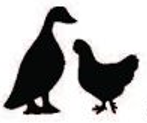
\includegraphics[scale=0.2]{../grafik/artikel/poultry}      & (G)     & Contains poultry (usually chicken).                                \\
        \hline
        \rule{0pt}{1cm+1ex}
\includegraphics[scale=0.2]{../grafik/artikel/pork}         & (S)     & Contains pork.                                                     \\
        \hline
        \rule{0pt}{1cm+1ex}
\includegraphics[scale=0.2]{../grafik/artikel/beef}         & (R)     & Contains beef.                                                     \\
        \hline
        \rule{0pt}{1cm+1ex}
\includegraphics[scale=0.2]{../grafik/artikel/veal}         & (K)     & Contains veal (meat from calves).                                  \\
        \hline
        \rule{0pt}{1cm+1ex}
\includegraphics[scale=0.2]{../grafik/artikel/lamb-mutton}  & (L)     & Contains lamb or mutton.                                           \\
        \hline
        \rule{0pt}{1cm+1ex}
\includegraphics[scale=0.2]{../grafik/artikel/venison-game} & (W)     & Contains venison or other game meat.                               \\
        \hline
        \rule{0pt}{1cm+1ex}
\includegraphics[scale=0.2]{../grafik/artikel/fish}         & (F)     & Contains fish.                                                     \\
        \hline
    \end{tabular}

    \begin{multicols}{2}
}{Johannes Alef, edited by Stefan Gries}

%\artikel{Wie wichtig ist studentisches Engagement?}
{Wahrscheinlich bist du neu an der Uni, vielleicht kommst du direkt aus der Schule, hast vorher gearbeitet oder eine Ausbildung gemacht. In dem Fall wird in den nächsten Wochen vieles neu für dich sein. Eine der größten Überraschungen ist hierbei oft, wie viel Mitspracherecht und Gestaltungsmöglichkeiten Studierende im Vergleich zu Schülerinnen und Schülern haben. Die Gestaltungsmöglichkeiten der Studierenden sind groß und sollten genutzt werden.
}{
    Viele Studierende scheinen ihr ganzes Studium mit Scheuklappen vor den Augen zu verbringen, denn alles was sie sehen ist ihr eigener Studienerfolg und der möglichst schnell angestrebte Abschluss. Dabei lohnt es sich gerade im Studium einmal über den eigenen Tellerrand hinaus zu schauen, denn als Student*in hast du eine Vielzahl an Möglichkeiten, um dich aktiv in den Unibetrieb einzumischen. Ein paar von ihnen will ich hier im Folgenden auflisten und etwas näher erläutern:\\

    \textbf{Fachschaft:}

    Falls du an unserer Ophase teilgenommen hast, dann war die Fachschaft höchstwahrscheinlich dein erster Kontakt zu anderen Studierenden. Als Fachschaft organisieren wir eine Vielzahl von Veranstaltungen (wie unter anderem die Ophase),  beobachten aktuelle Geschehnisse am Fachbereich, haben immer ein offenes Ohr für Probleme von Studierenden und entsenden Mitglieder in verschiedene Gremien am Fachbereich. So haben wir zum Beispiel ein Mitspracherecht, wenn es um die Berufung von neuen Professor*innen geht, oder wenn die Ordnung eines Informatik-Studiengangs geändert werden soll.

    Leider sind viele dieser Aktivitäten sehr arbeitsintensiv, sodass wir immer dankbar über alle sind, die ihren Teil dazu beitragen wollen, sei er auch noch so klein. Wenn du dich also für die Geschehnisse am Fachbereich interessierst, ist die Fachschaft eine tolle Anlaufstelle!

    Mehr über die Fachschaft erfährst du im Artikel "`Fragen und Antworten rund ums Thema Fachschaft"' und auf der Fachschaftswebseite\footnotemark[1].\\

    \textbf{Hochschulpolitik:}

    Wenn du dich für Politik interessierst und gerne die Universität aktiv mitgestalten möchtest, dann ist vielleicht auch die Hochschulpolitik etwas für dich. Du könntest zum Beispiel an den Treffen einer der vielen politischen Listen an der TU teilnehmen und wer weiß, vielleicht steht ja schon bei der nächsten Hochschulwahl auch dein Name auf den Stimmzetteln?

    Falls du lieber unabhängig bleibst, aber trotzdem politische Projekte mitgestalten willst, dann könntest du dich stattdessen auch für einen Referatsposten beim AStA bewerben. Die Referate werden von jährlich auf der AStA-Webseite\footnotemark[2] ausgeschrieben, du kannst aber auch einfach direkt mit deiner Projektidee auf den AStA zugehen.\\

    \textbf{Hochschulgruppen:}

    Weniger politisch, aber in keinem Fall weniger engagiert, sind auch die Hochschulgruppen an der TU. Du könntest dich zum Beispiel mit der HG Nachhaltigkeit für einen nachhaltigen Campus einsetzen oder bei "`Studieren ohne Grenzen"' dazu beitragen, dass junge Menschen auf der ganzen Welt Zugang zu Bildung erhalten.
    Doch das ist noch lange nicht alles: Ob Hackertreff, Sportclub, Chor, Orchester, Vernetzung mit internationalen Studierenden oder Filmkreis, hier ist wohl für jede*n etwas dabei.
    Eine Übersicht aller Gruppen findest du unter \footnotemark[3].\\

    \textbf{Lehre:}

    Letztendlich wird auch die Lehre zu einem gewissen Teil von Studierenden mitgestaltet. So leiten zum Beispiel erfahrene Studierende, die das jeweilige Fach schon abgeschlossen haben, als Tutor*innen deine Übungsgruppen. Darüber hinaus unterstützen sie als Assistent*innen die Professor*innen bei der Konzeption und Durchführung ihrer Lehrveranstaltungen und sind natürlich auch in aktuellen Forschungsprojekten involviert.
    Auch das Mentorensystem, welches du in deinem ersten Semester absolvieren musst und über das du an anderer Stelle noch mehr erfahren wirst, wäre ohne die vielen studentischen Mentor*innen nicht möglich.\\

    Wie du siehst, sind Studierende ein essentieller Bestandteil des Unibetriebs und sie haben durchaus auch die Macht, die Uni zu verändern. Vielleicht bist du ja nun selbst motiviert, dich neben dem Studium ein wenig zu engagieren und sorgst in Zukunft dafür, dass die Uni ein kleines bisschen besser wird.}
{Julian Haas}

\footnotetext[1]{\url{http://www.d120.de}}
\footnotetext[2]{\url{https://www.asta.tu-darmstadt.de}}
\footnotetext[3]{\url{https://www.tu-darmstadt.de/studieren/campusleben/engagement_student/hochschulgruppen.de.jsp}}

\newpage
\artikel{Questions and Answers Regarding the Fachschaft (student council)}
{In the previous articles you have already got a rough understanding of the Fachschaft. In this article you will learn what the Fachschaft really is, what the Fachschaft can do for you and how you can participate.
}{
\label{FSarticle}
\textbf{What does "die Fachschaft"? mean?}

The term Fachschaft originally means all students of a department, in this case the computer science department. Therefore, if you study at the computer science department, you are a part of the Fachschaft.\\

\textbf{Why "originally"?}

In everyday language use the students of computer science use the term "Fachschaft" for a few students who are actually part of the "active Fachschaft". A proper translation is departmental students representatives committee.\\

\textbf{What is the difference between the members of the Fachschaft and the rest of the students.?}

Primarily the members of the Fachschaft use their free time to help improve the studying situation for other students or at least prevent it from getting worse.\\

\textbf{And what can the Fachschaft actually do?}

If something happens at the department of computer science that has negative effects on your studies or if you have suggestions on how to improve the studying situation or your study program you can talk to the members of the Fachschaft about it. For example, if something is going wrong in a lecture, e.g. the organization is really bad, you (and maybe others who see the same problems) can talk to the Fachschaft and they can talk to the lecturer about how to improve the situation. This may of course take longer than talking to the lecturer yourself, but this way you can usually stay anonymous and since the Fachschaft has a good relationship to most lecturers, the matter will most likely be resolved faster. Additionally, the members of the Fachschaft can influence the politics of the department and bring the request to higher level of the hierarchy if necessary.\\

\textbf{Do I have to bring everything that bothers me about a lecture to the Fachschaft?}

Of course not. The Fachschaft mainly takes care of larger problems that affect many students or problems that need a lot of "lobbying" to be solved. If you only have a small issue it is normally much faster and less complicated to just talk to the lecturer about it yourself.\\

\textbf{How can I contact the Fachschaft if I have a severe problem with the studying situation?}

There are several ways: Most of the time you can find some members of the Fachschaft in the room of the Fachschaft S2$|$02 D120. Even if the person available can't directly help solve your issue they can usually tell you who you should talk to or inform the rest of the Fachschaft about it. If you don't want to go to D120 personally or simply aren't able to do so you can write an e-mail to the mailing list of the Fachschaft: wir@D120.de.\\

\textbf{You are mentioning the term "studying situation" all the time. What does the Fachschaft take care of exactly?}

The Fachschaft is active in the university politics, mainly (but not exclusively) on the departmental level: three representatives of the students are elected for the departmental council and can therefore influence decisions at the department. Furthermore some members of the Fachschaft are working in committees at the department, for example the QSL-committee that decides on the use of money given by the state Hessen for improving the studying situation, the committee for teaching and studying that discusses all subjects related to teaching. Naming and explaining all committees would take way too much space. If you want to see what committees members of the Fachschaft are active in you can take a look at \footnotemark[1].\\

\textbf{That sounds like serious business – is politics the only thing the Fachschaft does?!}

University politics is an important part of the work done by the Fachschaft, but not the only thing. Apart from the activities mentioned above there is a lot more that the Fachschaft organizes entirely or is at least partly responsible for. You are experiencing the most obvious one right now: the orientation phase is organized by the Fachschaft and many of the tutors are members of the Fachschaft. This booklet you are reading right now is a special issue of the journal of the students of computer science which is managed, organized and published during the semester by an editing staff that mostly consists of members of the Fachschaft. Currently, however, the journal is published only irregularly as there are too few people who are willing to write articles for the Inforz.\\
Additionally, the Fachschaft organizes the evaluation of the lectures every term and analyses the result. But the Fachschaft is also responsible for leisure time activities: every year the Fachschaft organizes the summer party and a St Nicholas party and the Fachschaft also organizes the regular game evening Games no Machines (GnoM) and RPGnoM, which are explained in the leisure part of this booklet. There are even more activities organized by the Fachschaft. You can get an overview here: \footnotemark[2].\\

\textbf{The word "organized" is in almost every sentence! Don't you need a lot of people for all these activities?}

Yes! A lot of people are needed and there are not enough to keep all this running. The entire work is done voluntarily and only a few students are motivated to invest some time into these things, as studying alone already takes up a lot of time. But imagine what your studies would be like if there was no orientation phase or nobody would try to ensure that bad lectures have to be improved. Mainly thanks to the work of the Fachschaft over the last years and decades the studying situation is as good as it is. But there is still plenty of room for improvement. A problem often not seen by normal students is that the members of the Fachschaft are students, too, who at some point finish their studies and leave the university. Because of that the Fachschaft always needs new members.\\

\textbf{With this much work to do it is no surprise that people are discouraged from helping.}

That is a very one-sided view. Of course there is a lot to do but on the other side this work can be split up into many small pieces if more people are helping. And there are also many small or one-time activities to be done which require some helping hands and don't need those helpers to get a deeper understanding of any subject handled by the Fachschaft.\\

\textbf{Really? And how do I get to know about these events so that I may help some time?}

There are several ways to get information about these events. You can always ask members of the Fachschaft in room S2$|$02 D120 about current activities. If you want to get a deeper understanding of the work done by the Fachschaft, then the meeting of the Fachschaft, which takes place every Wednesday at 18:00, is a good place. In these meetings all currently important topics are discussed. Please note that due to the fact that currently there are only German members of the Fachschaft, the meetings are held in German. So it would be good to understand some German to be able to follow the conversation. If you don't speak German very well it is probably easier to ask a member of the Fachschaft to explain the discussed matters to you a few days after the meeting. If there is no meeting held in the room of the Fachschaft you can always spend some time there and get informed. Other possibilities to get informed are the web page of the Fachschaft \footnotemark[3], the blog of the Fachschaft (called "das Wesentliche") \footnotemark[4], the facebook page of the Fachschaft \footnotemark[5] or the Twitter-Account @d120de \footnotemark[6]. Of course most of these are in German for the above mentioned reason. If you want to participate from time to time in a certain area you can also register yourself on one of the mailing lists. An overview can be found here: \footnotemark[7].
}
{Stefan Gries\\
edited by Julian Haas\\
edited and translated by Johannes Alef}


\footnotetext[1]{\url{http://www.d120.de/gremien/}}
\footnotetext[2]{\url{https://www.d120.de/en/students/}}
\footnotetext[3]{\url{http://www.d120.de}}
\footnotetext[4]{\url{http://daswesentliche.d120.de/}}
\footnotetext[5]{\url{https://www.facebook.com/d120.de}}
\footnotetext[6]{\url{https://twitter.com/d120de}}
\footnotetext[7]{\url{http://www.d120.de/mailman/listinfo}}

%\newpage


%\vfill
%\bildmitunterschrift{../grafik/comics/phishing_license}{width=\textwidth}{}{xkcd.com}

%\artikel{Politik an der Uni?}
{Politik gibt es nicht nur in der großen Welt, sondern auch an Hochschulen. Hier ein kleiner Überblick, welche Gremien wofür stehen und was sie leisten.
}{
    \noindent\textbf{Universitätswahl}\\
    Wie in der Bundes- und Landespolitik auch, hängt der Erfolg der Hochschulpolitik entschieden davon ab, dass sich Leute daran beteiligen.\\
    Dies kannst du auf 2 verschiedenen Wegen tun: Entweder du engagierst dich selbst in den Gremien, oder du nutzt einfach die jährlichen Hochschulwahlen im Sommersemester um deiner Stimme Ausdruck zu verleihen.\\
    Aber warum wählen? Die Wahl ist deine Möglichkeit, in die Hochschulpolitik einzugreifen und etwas zu verändern. Mit deiner Stimmabgabe wählst du dabei nicht nur eine Liste oder Person, du unterstützt auch alle anderen, die dich in diesem Gremium vertreten; denn es ist ein Unterschied, ob die Vertreterinnen und Vertreter von fünf Prozent der Studierenden gewählt wurden oder eben von 50 Prozent.

    Es gibt also mehr als einen guten Grund, zur Wahl zu gehen. Dennoch haben wir in den letzten sechs Jahren ausbaufähige Teilnahmezahlen gehabt. Hier die Wahlbeteiligung der letzten Wahlen:\\

    \begin{tabular}{ll}
        2019 & 12,8\% \\
        2018 & 11,9\% \\
        2017 & 16,9\% \\
        2016 & 15,2\% \\
        2015 & 13,5\% \\
        2014 & 17,9\% \\
    \end{tabular}
    \\\\
    Es waren immer relativ niedrige Ergebnisse, deswegen ist es besonders wichtig, dass du dich an der Wahl beteiligst. Wir werden früh genug darauf aufmerksam machen, sodass du sie nicht verpassen wirst.

    \noindent
    \subsection*{Gremien am Fachbereich:}
    \textbf{Fachbereichsrat}\\
    Der Fachbereichsrat, meist nur FBR genannt, ist das höchste Gremium am Fachbereich. Er behandelt Angelegenheiten von grundsätzlicher Bedeutung für den Fachbereich. Der FBR ist zuständig für

    \begin{itemize}
        \item Erlass der Ordnungen der Studiengänge
        \item Planung der Lehrveranstaltungen
        \item Zusammensetzung von Berufungskommissionen für neue Professor*innen
        \item Ausstattung der Fachgebiete
        \item Abstimmung der Forschungsvorhaben
        \item Wahl des Dekans bzw. der Dekanin
    \end{itemize}

    Dem FBR Informatik gehören sieben Professor*innen, zwei WiMis (Wissenschaftliche Mitarbeiter*innen), ein*e administrativ-technische*r Mitarbeiter*in und drei Studierende an. Gewählt werden diese von ihren jeweiligen Gruppen.

    Wir haben zwar keine Mehrheit, aber das bedeutet nicht, dass wir keinen Einfluss in diesem Gremium hätten. \\

    \noindent\textbf{Fachschaftsrat}

    Der Fachschaftsrat (FSR) besteht nur aus Studierenden und ist so etwas wie die "`gewählte Fachschaft"'. An unserem Fachbereich sind das 9 Personen, doch wir machen keinen wirklichen Unterschied zwischen gewählten Fachschaftler*innen und solchen, die sich einfach so beteiligen wollen. Jede*r ist herzlich dazu eingeladen, mitzuarbeiten.\\

    Die Fachschaft vertritt die Interessen aller Informatikstudierenden und setzt sich stetig dafür ein, das Informatikstudium an der TU noch besser zu machen. Dazu trifft sich die Fachschaft normalerweise zu wöchentlichen Sitzungen (derzeit Mittwochs um 18:00 Uhr) und in verschiedenen Arbeitskreisen und Ausschüssen. Wir entsenden außerdem Leute zur Fachschaftenkonferenz, wo einmal im Monat Probleme zwischen allen Fachschaften der TU geklärt werden, und zur KIF, der Konferenz der deutschsprachigen Informatikfachschaften.\\

    Sie ist außerdem Ansprechpartnerin bei Fragen und Problemen rund um das Studium. Auch Probleme mit Professor*innen können hier durchaus angesprochen werden.

    Mehr zur Fachschaft und zum Fachschaftsrat findest du im Artikel "`Fragen und Antworten rund ums Thema Fachschaft"', oder du besuchst uns einfach mal in Raum D120.

    \subsection*{Uniweite Gremien:}
    \noindent\textbf{Universitätsversammlung}

    In der Universitätsversammlung (UV) sind die Studierenden mit 15 Mitgliedern vertreten. Ihnen stehen 31 Professor*innen, zehn wissenschaftliche Mitarbeiter*innen und  fünf administrativ-technische Mitarbeiter*innen aller Fachbereiche gegenüber.

    \noindent Wie bei allen universitätsweiten Gremien gibt es hier Listenwahl, keine Personenwahl. Auf jeder Liste stehen Vertreterinnen und Vertreter verschiedener Fachbereiche, einige Listen verfolgen die Ziele ihrer "`großen Mutterparteien"', andere dagegen sind unabhängig.

    Die Aufgaben der UV sind die Wahl des Präsidiums und die Verabschiedung von Ordnungen, die die ganze Universität betreffen. Außerdem wählt sie die Mitglieder des Senats, darunter befinden sich auch vier studentische.\\

    \noindent\textbf{Studierendenparlament}

    Das Studierendenparlament (StuPa) besteht aus 31 studentischen Mitgliedern, die per Listenwahl gewählt werden. Seine Aufgabe ist vor allem die Wahl und Kontrolle des Allgemeinen Studierendenausschusses (AStA) sowie Verwaltung des Haushaltes der Studierendenschaft.\\

    \noindent\textbf{Senat}

    Der Senat der TU Darmstadt überwacht die Geschäftsführung des Präsidiums und berät es in Angelegenheiten, die die Struktur, die Entwicklungs- und Bauplanung, den Haushalt, die Forschung, die Lehre oder das Studium betreffen. Der Senat hat 20 Mitglieder, die von der Universitätsversammlung gewählt werden. Unter ihnen sind vier Studierende.\\

    \noindent\textbf{AStA}

    Der Allgemeine Studierendenaussschuss (AStA) ist die Vertretung der Studierenden auf Hochschulebene und wird größtenteils vom Studierendenparlament gewählt.
    Auf politischer Ebene setzt sich der AStA für die Interessen aller Studierenden ein und ist außerdem verantwortlich für eine Vielzahl an Serviceangeboten.
    Mehr über den AStA erfährt du im nächsten Artikel.

}
{Julian Haas}

\bildmitunterschrift{comics/two_party_system}{width=\textwidth}{}{xkcd.com}

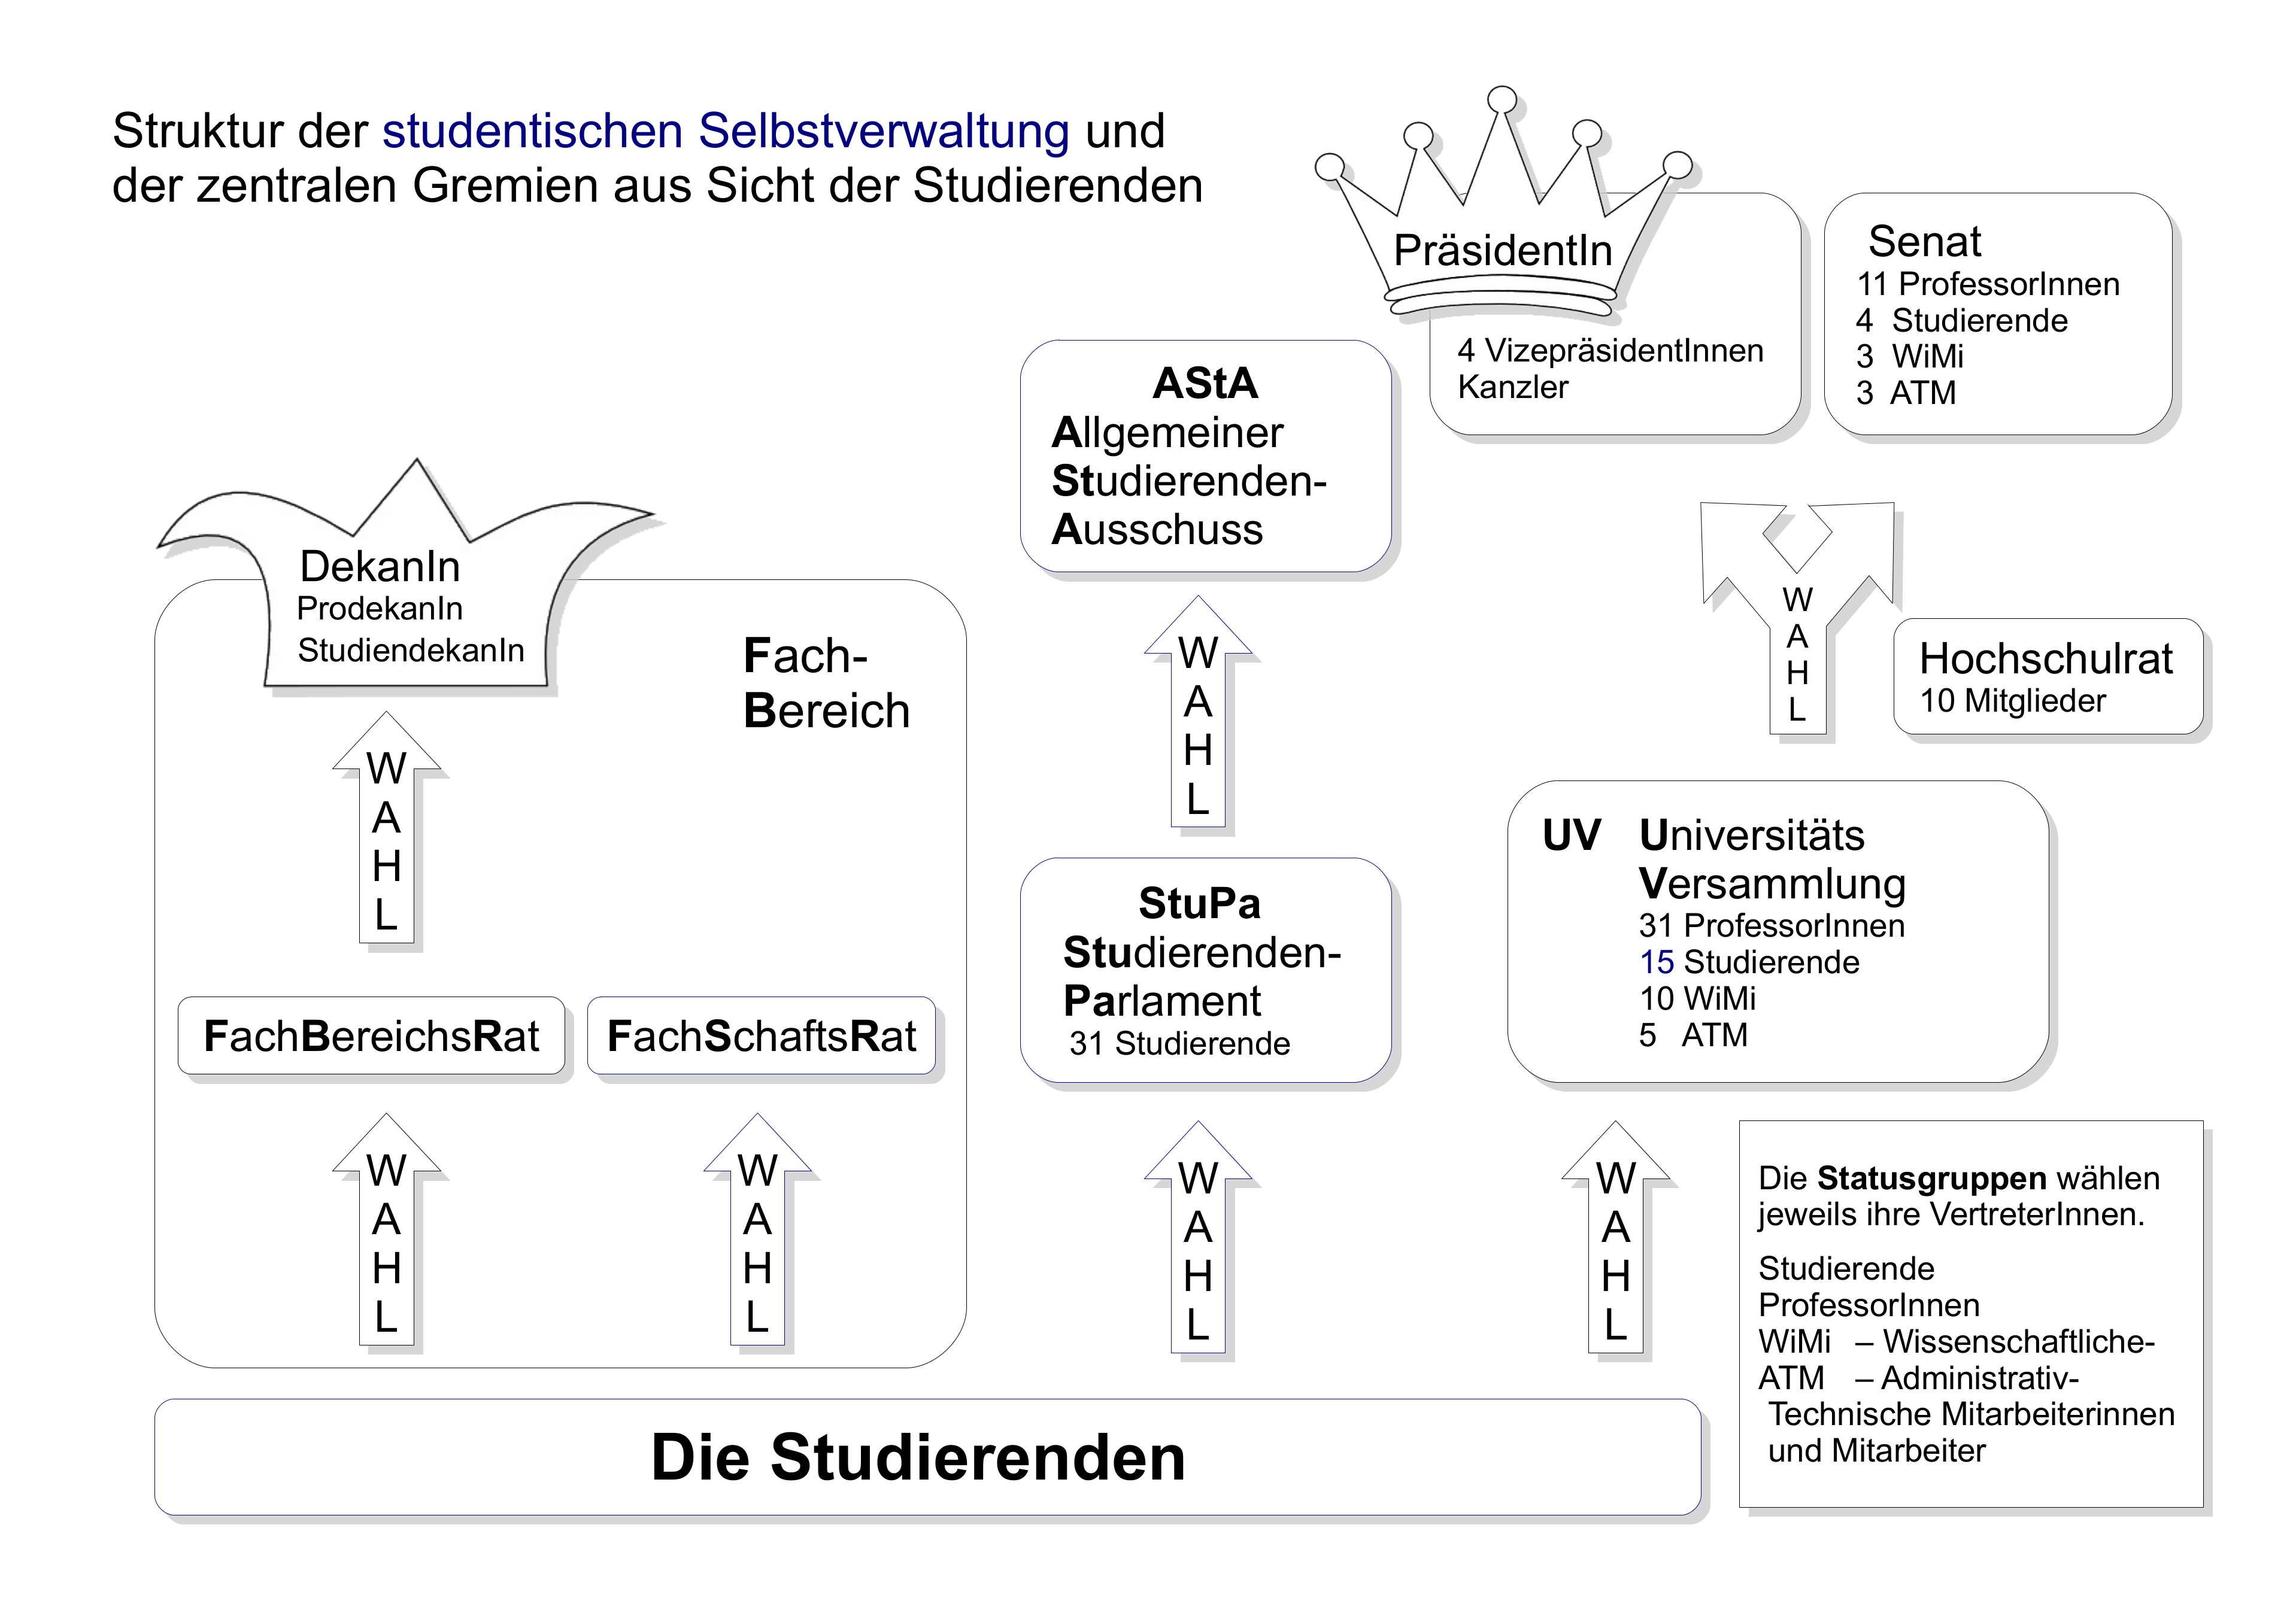
\includegraphics[angle=270,totalheight=17cm]{artikel/hopo2}

\newpage

%\artikel{Der AStA der TU Darmstadt}
{Der Allgemeine Studierendenausschuss (AStA) ist die oberste Vertretung aller Studierenden auf Universitätsebene. Darüber hinaus ist er Ansprechpartner bei Problemen und bietet für Studierende etliche Service- und Beratungsangebote.
    Wer der AStA eigentlich ist und was er alles so macht, erfährst du in diesem Artikel.
}{
    \noindent\textbf{Aufgaben des AStA}\\
    Die Aufgaben des AStA sind vielfältig und leiten sich aus den Aufgaben der Studierendenschaft ab, die nach §3 der Satzung der Studierendenschaft definiert sind:

    \begin{itemize}
        \item	Die Vertretung der Gesamtheit ihrer Mitglieder im Rahmen ihrer gesetzlichen Befugnis.
        \item	Die Wahrnehmung der hochschulpolitischen Belange ihrer Mitglieder.
        \item	Die Wahrnehmung der wirtschaftlichen und sozialen Belange der Student*innen. Die Zuständigkeit des Studierendenwerkes (StuWe) oder anderer Träger bleibt unberührt.
        \item	Die Pflege überregionaler und internationaler Studierendenbeziehungen.
        \item	Die Förderung der politischen Bildung und des Verantwortungsbewusstseins von Student*innen für ihre Rolle als Staatsbürger*innen. Hierzu gehört auch die Förderung eines wissenschaftlich fundierten, kritischen Verständnisses der Student*innen von ihrer jetzigen und künftigen Tätigkeit und der Rolle von Wissenschaft und Technik in der Gesellschaft.
        \item	Die Unterstützung kultureller und musischer Interessen der Student*innen.
    \end{itemize}

    Das mag erst einmal alles sehr förmlich und theoretisch klingen, doch tatsächlich arbeiten täglich AStA-Referentinnen und -Referenten daran, die Studienbedingungen an der TU zu verbessern. Der AStA engagiert sich zum Beispiel für Studierende in sozialen Notsituationen und steht im ständigen Kontakt mit der Universitätsleitung. Er sorgt mit seinen Gewerben und Veranstaltungen für mehr Kulturangebote in Darmstadt und ist zum Beispiel auch dafür verantwortlich, dass es das Semesterticket in seiner jetzigen Form überhaupt gibt.
    Du siehst also: Der AStA hat durchaus auch Einfluss auf deinen Studienalltag.\\

    \bildmitunterschrift{artikel/eule_final_orange}{width=\linewidth}{}{}


    \noindent\textbf{Doch wie kommt man eigentlich in den AStA?}\\
    Der AStA besteht größtenteils aus Referenten und Referentinnen, die jedes Jahr vom Studierendenparlament gewählt werden. Neben diesen gewählten Referaten gibt es inzwischen auch viele eingestellte Referate, die von engagierten Studierenden geleitet werden, die mit einem tollen Projekt zum AStA gekommen sind und dann für ihr jeweiliges Referat eingestellt wurden.

    Aktuell gibt es zum Beispiel Referate zum Thema: Nachhaltigkeit, Queer, Feminismus, Mobilität, Inklusion, Familienförderung und noch vieles mehr.\\
    \columnbreak

    \subsection*{Angebote des AStA im Detail}

    Neben dem politischen Engagement ist der AStA wie eingangs schon erwähnt für viele Servicangebote zuständig. Hier eine kleine Auswahl.\\

    \noindent\textbf{Fahrradverleihsystem Call a Bike}\\
    Für alle Darmstädter Studierenden ist beim Leihfahrradsystem "`Call a Bike"' der Deutschen Bahn jeweils die erste Stunde jeder Fahrt kostenlos. Und das auch noch deutschlandweit! Die Räder können ganz einfach an einer Station entliehen und an einer beliebigen anderen Station zurückgegeben werden. In Darmstadt gibt es inzwischen über 30 Stationen und eine liegt direkt am Piloty. Mehr zum Angebot unter \footnotemark[1].\\

    \noindent\textbf{RMV-AStA Semesterticket}\\
    Dein Studienausweis ist gleichzeitig dein Semesterticket und bietet kostenlose Fahrten mit dem öffentlichen Nahverkehr im gesamten RMV-Gebiet und teilweise auch im Übergangsgebiet (siehe Grafik auf der nächsten Seite). Die Konditionen für dieses Ticket verhandelt regelmäßig der AStA und er ist auch dein Ansprechpartner bei allen Fragen um das Ticket (z.B. Ticket-Erstattung bei Auslandssemestern). Mehr unter \footnotemark[2].\\

    \noindent\textbf{AStA-Büros}\\
    Die AStA-Büros in der Stadtmitte (S1$|$03-62) und auf der Lichtwiese (L3$|$01-70) sind deine erste Anlaufstelle, wenn du Fragen zum AStA, den Angeboten oder auch generell zu Geschehnissen in der Universität hast. Auch wenn du dich selbst gerne einbringen würdest oder ein Projekt starten willst, bist du hier richtig. Lagebeschreibung und Öffnungszeiten unter \footnotemark[3].\\

    \noindent\textbf{Beratungsangebote}\\
    Der AStA organisiert und vermittelt kostenlose Erstberatung zu vielen verschieden Themen. Im Detail sind dies derzeit die BAföG- und Sozialberatung, die Rechtsberatung durch erfahrene Anwälte, die Mietrechtsberatung, die Arbeitsrechtsberatung in Zusammenarbeit mit dem DGB und die Sprechstunde für internationale Studierende. Wenn du nicht genau weißt, an welche der vielen Beratungsstellen du dich eigentlich mit deinem Problem wenden sollst, dann frag am Besten einfach mal in einem der AStA-Büros nach. Infos und aktuelle Sprechzeiten findest du unter \footnotemark[4].\\

    \noindent\textbf{Kultur-Kooperationen}\\
    Aus dem Semesterbeitrag gehen 0,50 \euro~ an das Staatstheater Darmstadt. Dafür hat jede*r Studierende die Möglichkeit, kostenlos Restkarten für Theater, Konzerte, Ballett, Opern oder Musicals im Staatstheater zu bekommen. Wie es geht, steht unter \footnotemark[5].\\

    \noindent\textbf{Studentische Gewerbe}\\
    Neben den Serviceangeboten ist der AStA auch zuständig für eine Vielzahl an Gewerben, welche größtenteils von Studierenden verwaltet werden. Direkt auf dem Campus Stadtmitte findet man das Kulturcaf\'e 806qm und die Fahrradwerkstatt 20$^\circ$. Dazu kommen noch der Schlossgarten (der Biergarten auf der Bastion des Schlosses) und der Nachtclub Schlosskeller, der für seine Musik abseits des Mainstream bekannt ist. Auf dem Campus Lichtwiese betreibt der AStA außerdem einen Papierladen.

    Alle weiteren Infos rund um den AStA und dessen weitere Angebote findest du auf der AStA-Homepage unter \footnotemark[6].
}
{Julian Haas}

\footnotetext[1]{\url{https://www.asta.tu-darmstadt.de/asta/de/angebote/call-a-bike}}
\footnotetext[2]{\url{https://www.asta.tu-darmstadt.de/asta/de/angebote/semesterticket}}
\footnotetext[3]{\url{https://www.asta.tu-darmstadt.de/asta/de/angebote/bueros}}
\footnotetext[4]{\url{https://www.asta.tu-darmstadt.de/asta/de/angebote/beratung}}
\footnotetext[5]{\url{https://www.asta.tu-darmstadt.de/asta/de/angebote/staatstheater}}
\footnotetext[6]{\url{https://www.asta.tu-darmstadt.de}}

\newpage

%\newpage
\artikel{Public transport with your student ID}
{How to use the public transport without paying fees - because you have already paid them.}
{The AStA (Allgemeiner Studierendenausschuss - \textit{general committee of students}) has arranged that you can use your student ID as a public transport ticket within quite a huge area around Darmstadt (i.e. almost all of Hessen) -- without additional fees, as you already paid for these by enrolling at TU Darmstadt.
    That means you do not have to pay in order to take a regional train to Frankfurt, but you still have to pay extra for transportation using long-distance trains like ICE (inter-city express) or IC (inter-city)/EC (euro-city) trains.
    The image on the next page shows you in which area you can use your student ID as a public transport ticket.
    You need to have your regular ID as well as you student ID with you in order for your student ID to be recognised as a public transport ticket.\\

    \noindent\textbf{Travel in Germany by bus and train}
    However, you may want to travel through through more of Germany than Hessen only.
    In that case you can buy train tickets via Deutsche Bahn (the German train services). \footnotemark[1].
    You can basically obtain two types of tickets:
    The standard ticket allows you to travel within the day of booking on the route you have selected.
    In this case, iIf you order an ICE Ticket from Frankfurt to Stuttgart and your train stops in Heidelberg, you can exit the train in Heidelberg, do a bit of sightseeing and resume your travel to Stuttgart on the same day.
    In addition to the regular price tickets, the Deutsche Bahn offers tickets at special discounts, called Sparpreise.
    If you obtain one of the latter, you are usually train-bound, which means you have to take the exact sequence of trains listed in your ticket and will get into trouble if you intend to take a different train.
    If you don't feel overly confident about booking a trip online or via ticket machine, you can also still visit a travel centre in any larger train station (e.g. Darmstadt's central station) and find helpful staff to guide you through the process.

    In recent years, several long-distance bus services like \footnotemark[2] \footnotemark[3] have established themselves in Germany.
    These are usually cheaper than taking a train, but often take a little longer than the former.
    There are a few long-distance bus routes passing through Darmstadt and several more stopping in Frankfurt, which connect to nearly every larger city in Germany as well as some destinations in neighbouring countries.
}
{Anna-Katharina Wickert\\Stefan Gries}

\footnotetext[1]{\url{https://www.bahn.de/}}
\footnotetext[2]{\url{https://www.flixbus.de/}}
\footnotetext[3]{\url{https://meinfernbus.de/}}

\newpage

\artikel{Validity of your ticket}{}{
    \end{multicols}
    \vfill
    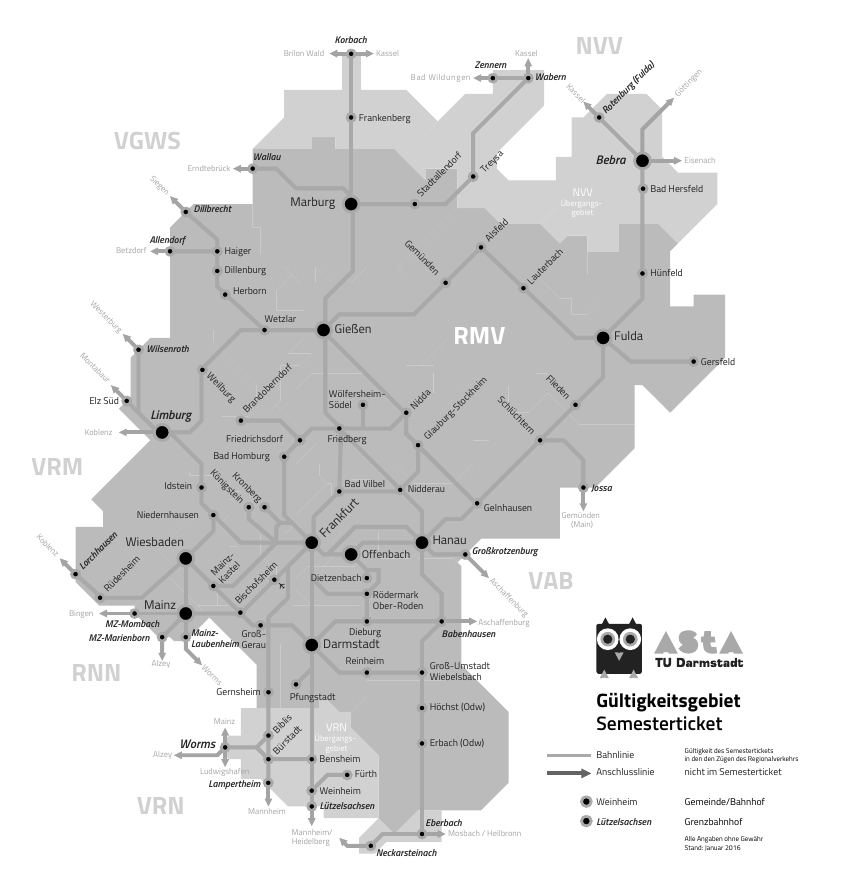
\includegraphics[width=\textwidth]{artikel/semesterticket}
    \vfill
    \begin{multicols}{2}
}{}


\kapitel{Leisure}{wesen/wesen_grill_hochzeitsturm}
{%Das Semester ist eine unangenehme Unterbrechung der Ferien
}
{%Johann Jakob Nöggerath (auch Noeggerath), /1788 - 1877), dt. Mineraloge und Geologe, ab 1814 Königlich Preußischer Geheimer Baurat
}

\artikel{Living in Darmstadt}
{Just studying isn't everything: Students should also find time for leisure activities. This section guides you through what Darmstadt has to offer.
}{
    The previous pages were all about the academic side of your studies. But there is another important part: leisure time. It serves as counter balance to an exhausting day and replenishes energy to take on the next day. It also helps us to clear our head from time to time.

    That's why it is so important, especially during strenuous weeks, to plan for regular breaks and leisure time. Studying is important but a clear head makes it a lot easier. Maybe an assignment needs to be finished - if you don't wait to start on the last day before the deadline you won't have to work on it all night.

    Everyone has their own idea of how to spend their leisure time but a good mix consisting of social interactivity (parties, game nights, cooking nights, etc.) and doing some sports is always recommended. The following pages shall help you to get to know what Darmstadt has to offer and to create your own personal leisure time.
}
{Tobias Freudenreich, Martin Tschirsich, Stefan Gries \\ edited and translated by Nils M.}

\artikel{All switches off}
{One of the most pleasant options to spend one's leisure time is to turn all switches off and just relax which is especially pleasant outside on warmer days during the summer.
}{
    Darmstadt's inhabitants find quite a few hidden gems in their surroundings that sometimes even the mature students don't know about: In the north of the city lies the Citizens Park (German: Bürgerpark) right behind the Nordbad (an indoor (winter)/outdoor (summer) swimming pool), in the south at Heidelberger Street is the Prince-Emil-Garden and the Orangerie, and close to the train station to the east (Ostbahnhof) one can find the Zoo "Vivarium" and the Rosenhöhe (another smaller park).
    The Herrngarten, Darmstadt's largest park can't be missed by computer science students as it is right behind the Piloty-Building. Another point of interest is the Mathildenhöhe (park) featuring the towns landmark, the wedding tower, and its regular art and cultural program.

    During the hot summer months you can cool down in one of the many swimming pools and lakes in and around Darmstadt. Most interesting for students beside the above mentioned Nordbad (very cheap for students) is the university's own outdoor pool located in the south right beside the University Sports Center. This pool is free of charge for students (bring your student ID) and is in range of the university's WiFi network. Perfect for soaking up the sun while studying a bit and going for a dip every once in a while.
    If you prefer to swim in lakes, the Woog, located fairly central in the city, is for you. There is also a few other lakes outside of Darmstadt, namely the Arheilige Mühlchen and the Grube Prinz von Hessen, both free of charge.
}
{Tobias Freudenreich, Martin Tschirsich, Stefan Gries \\ edited and translated by Nils M.}
\newpage

\artikel{Sports}
{Exercise is a great way to clear your head and promote creativity: It usually is very social but everyone has to find their own favorite type of exercise.
}{
Someone feeling competitive might enjoy ball sports or martial arts more than someone who'd rather have a quiet time and takes the bike to Castle Frankenstein or goes jogging.
Still undecided? Take a look at the catalogue of the University Sports Center. They offer about 90 different sports courses and exercise activities every week for students and employees of the TU Darmstadt. Some examples are fitness courses like Aerobic or Zumba, ball sports like badminton or Football but also exotic sports like Canoe-Polo, Underwater-Rugby or Ultimate Frisbee.
Some courses may cost a small fee but most of them are free of charge to participate. You can find registration forms and more information here: \footnotemark[1] . Unfortunately, the website is currently only offered in German, so if you need help registering or getting more information, just ask anyone in the Fachschaft (Room D120 in the Piloty-Building) or someone else that understands German. The University Sports Center also operates a golf practice course and a gym. From time to time they offer exclusive workshops like diving or step dance.
One of the more popular offers is the outdoor pool, especially during the summer, which is free of charge for students.
Each term there are internal championships in various sports like Football, Badminton or Volleyball. Those are more for fun but if you want to get real competitive, you can try-out for participation in the German University Sports Federation Championships. Information about these championships can be found on the websites of the University Sports Center \footnotemark[1] and the German University Sports Federation \footnotemark[2] respectively.
Due to limited space the gym fills up quickly, so register early if you want to get a membership! Other offers do fill up quickly, too in which case it might be preferable to join a local sports team instead. Often, these clubs offer memberships at discounted prices for students as well.
Darmstadt also offers a skating rink and a climbing forest as well as several parks and indoor/outdoor swimming pools.
If you're up for a challenge, you can join the local Jugger team, Pink Pain \footnotemark[3] . Their web presence is only in German but the team consists of quite a few computer science students and we're always happy to introduce you to the world of Jugger. 
}
{Tobias Freudenreich, Martin Tschirsich, Stefan Gries \\ edited and translated by Nils M.}

\footnotetext[1]{\url{http://www.usz.tu-darmstadt.de}}
\footnotetext[2]{\url{http://www.adh.de/en.html}}
\footnotetext[3]{\url{http://www.jugger-darmstadt.de}}
\newpage

%\input{inhalt/freizeit/darmstadt_kulinarisch_engl}
%\input{inhalt/freizeit/abendprogramm_engl}
\artikel{GnoM - The LAN party without a power supply}
{Travel through time with the Fachschaft of computer science and rediscover long lost traditions.
}{
    When even the most ingrained computer scientists leave their coffee cups behind and move towards the upper levels, away from the computer pool, there must be something special going on.
    They're migrating towards Room E202 in the Piloty building, armed with candy and mysterious cardboard boxes without USB-Ports or power supplies.
    Outsiders might wonder what computer scientists may intend to do with such boxes. The answer is easy: They just want to play.
    Upon arrival in room E202, even mathematics and physics students can sometimes be seen around.
    Some long-term student may feel like being transported back in time, back to days before the invention of electricity, and is tempted to light a candle.
    But that is not necessary: the no-power-supply rule only applies to entertainment electronics. This is "Games no Machines", or in short -- GnoM.
    For $10100_2$ years already, the Fachschaft of computer science organizes this legendary evening where PCs are left in the pool, and only good old board and card games are being pulled off the dusty shelf.
    Everyone is welcome and invited to participate and see for themselves how much fun a LAN party without power can be.
    Of course, one can bring their own games as well.
    More information about the scheduled dates can be obtained from the GnoM mailing list \footnotemark[1], the Fachschaft's forums \footnotemark[2], the blog "das Wesentliche" \footnotemark[3] and especially (as these websites are mostly in German) everywhere helpful members of the Fachschaft can be found, primarily in the Fachschaft's room, D120.
    General information, again in German, can be found here: \footnotemark[4].
}
{
    Alexandra Weber\\edited by Julian Haas\\edited and translated by Nils M.\\translation edited by Stefan Gries
}

\footnotetext[1]{\url{http://www.d120.de/mailman/listinfo/gnom}}
\footnotetext[2]{\url{https://www.fachschaft.informatik.tu-darmstadt.de/forum/}}
\footnotetext[3]{\url{http://daswesentliche.d120.de}}
\footnotetext[4]{\url{http://www.d120.de/gnom}}

\artikel{RPGnoM}
{GnoM's little sibling}
{For $1_2$ year already, GnoM (again) has a little brother: RPGnoM.
    This group focuses on role-playing games, the respective gaming evenings take place in the same rooms as the regular GnoM.
    The primary difference between board games and role-playing games is that, while still based on a set of game rules, role-playing games emphasise group-focused interactive storytelling over traditional competitive game mechanisms.
    RPGnoM evenings are sheduled via survey and then a date will be published by means of the dedicated mailing list \footnotemark[5].
    On most dates, the participants organize an order of food so that players don't go hungry.
    General information, again in German, can be found here: \footnotemark[6].
}
{
    Anna-Katharina Wickert,\\Stefan Gries
}

\footnotetext[5]{\url{http://www.d120.de/mailman/listinfo/rpgnom}}
\footnotetext[6]{\url{https://www.d120.de/de/studierende/rpgnom/}}

%\vfill
%\bildmitunterschrift{comics/nerd_sniping}{width=\textwidth}{}{xkcd.org}
%\newpage


%\bildmitunterschrift{comics/old_files}{height=17cm}{}{xkcd.org}

\kapitel{For Look-up}{}
{Here you can look up some important information.}{}

\addsec{Dictionary}

The following tables give translations for some study-relevant vocabulary.
The first table is German-Englisch, the second one is English-German.

\begin{longtable} {|p{.5\linewidth}|p{.5\linewidth}|}
    \hline
    \textsc{German}                     & \textsc{English}                                               \\
    \hline
    \hline
    abschließen                         & complete                                                       \\
    \hline
    Abschlussarbeit                     & thesis                                                         \\
    \hline
    Abschlusszeugnis                    & degree certificate                                             \\
    \hline
    anerkennen                          & to transfer credits                                            \\
    \hline
    Anerkennung                         & transfer of credit(s)                                          \\
    \hline
    Anmeldefrist                        & registration deadline                                          \\
    \hline
    Anmeldung                           & registration                                                   \\
    \hline
    Ausführungsbestimmungen             & implementation terms                                           \\
    \hline
    Bachelorpraktikum                   & Practical lab for Bachelors                                    \\
    \hline
    Beratungssystem                     & advisory system                                                \\
    \hline
    Bescheinigung                       & certificate                                                    \\
    \hline
    Dozent                              & lecturer                                                       \\
    \hline
    einbringen                          & include                                                        \\
    \hline
    Einführungsveranstaltung            & introductory course                                            \\
    \hline
    Einschreibung                       & enrollment                                                     \\
    \hline
    Exmatrikulation                     & deregistration                                                 \\
    \hline
    Fachbereich Informatik              & Department of Computer Science                                 \\
    \hline
    Fachschaft                          & departmental student representative committee, student society \\
    \hline
    Grundlagenveranstaltungen           & basic course                                                   \\
    \hline
    kanonische Einführungsveranstaltung & canonical introductory course                                  \\
    \hline
    Kommilitone                         & fellow student                                                 \\
    \hline
    Leistungen                          & academic achievements                                          \\
    \hline
    Leistungsspiegel                    & list of achievements                                           \\
    \hline
    Matrikelnummer                      & registration number                                            \\
    \hline
    Nebenvereinbarung                   & special terms attached to the Learning Agreement               \\
    \hline
    nur in deutscher Sprache vorhanden  & in German language only                                        \\
    \hline
    Orientierungsphase                  & orientation days                                               \\
    \hline
    Orientierungsveranstaltungen        & orientation events                                             \\
    \hline
    Pflichtbereich                      & category of required courses                                   \\
    \hline
    Pflichtveranstaltung                & required course                                                \\
    \hline
    Prüfung absolvieren                 & take an exam                                                   \\
    \hline
    Prüfung bestehen                    & pass                                                           \\
    \hline
    Prüfungskomission                   & Examination Committee                                          \\
    \hline
    Prüfungsleistung                    & examination achievement                                        \\
    \hline
    Prüfungsordnung                     & examination regulations                                        \\
    \hline
    Prüfungsplan                        & Examination Plan                                               \\
    \hline
    Prüfungssekretariat                 & Examination Office                                             \\
    \hline
    Referat Internationale Beziehungen  & International \& External Affairs Office                       \\
    \hline
    Registrieren                        & register                                                       \\
    \hline
    Service für andere Fachbereiche     & service for other departments                                  \\
    \hline
    Spezialveranstaltungen              & special courses                                                \\
    \hline
    Sprechstunde                        & office hour                                                    \\
    \hline
    Studienberatung                     & Student Advisory Service                                       \\
    \hline
    Studienbüro                         & Office of Study Programs and Examination                       \\
    \hline
    Studiendekan                        & Dean for Student Affairs, dean of studies                      \\
    \hline
    Studiendekanat                      & Dean's Office for Student Affairs                              \\
    \hline
    Studiengang                         & study program                                                  \\
    \hline
    Studienleistung                     & coursework                                                     \\
    \hline
    Studierendensekretariat             & Office of Student Affairs                                      \\
    \hline
    Studium                             & studies                                                        \\
    \hline
    Studium abschließen                 & graduate                                                       \\
    \hline
    Urlaubssemster                      & semester on leave                                              \\
    \hline
    Vertiefungsveranstaltungen          & advanced level courses                                         \\
    \hline
    vorgezogene Masterleistungen        & preponed Master courses                                        \\
    \hline
    Vorlesungsverzeichnis               & course schedule                                                \\
    \hline
    vorläufige Anerkennung              & preliminary ...                                                \\
    \hline
    Wahlbereich                         & category of elective courses                                   \\
    \hline
    Wahlpflichtbereich                  & category of required elective courses                          \\
    \hline
    Wahlpflichtveranstaltung            & required elective course                                       \\
    \hline
    Zeugnis                             & report                                                         \\
    \hline
    Zuordnung                           & subject classification                                         \\
    \hline
    Zwangsexmatrikulation               & compulsory deregistration                                      \\
    \hline
\end{longtable}






\begin{longtable} {|p{.5\linewidth}|p{.5\linewidth}|}
    \hline
    \textsc{Englisch}                                              & \textsc{German}                     \\
    \hline
    \hline
    academic achievements                                          & Leistungen                          \\
    \hline
    advanced level courses                                         & Vertiefungsveranstaltungen          \\
    \hline
    advisory system                                                & Beratungssystem                     \\
    \hline
    basic course                                                   & Grundlagenveranstaltungen           \\
    \hline
    canonical introductory course                                  & kanonische Einführungsveranstaltung \\
    \hline
    category of elective courses                                   & Wahlbereich                         \\
    \hline
    category of required courses                                   & Pflichtbereich                      \\
    \hline
    category of required elective courses                          & Wahlpflichtbereich                  \\
    \hline
    certificate                                                    & Bescheinigung                       \\
    \hline
    complete                                                       & abschließen                         \\
    \hline
    compulsory deregistration                                      & Zwangsexmatrikulation               \\
    \hline
    coursework                                                     & Studienleistung                     \\
    \hline
    course schedule                                                & Vorlesungsverzeichnis               \\
    \hline
    Dean for Student Affairs, dean of studies                      & Studiendekan                        \\
    \hline
    Dean's Office for Student Affairs                              & Studiendekanat                      \\
    \hline
    degree certificate                                             & Abschlusszeugnis                    \\
    \hline
    Department of Computer Science                                 & Fachbereich Informatik              \\
    \hline
    departmental student representative committee, student society & Fachschaft                          \\
    \hline
    deregistration                                                 & Exmatrikulation                     \\
    \hline
    enrollment                                                     & Einschreibung                       \\
    \hline
    examination achievement                                        & Prüfungsleistung                    \\
    \hline
    Examination Committee                                          & Prüfungskomission                   \\
    \hline
    Examination Office                                             & Prüfungssekretariat                 \\
    \hline
    Examination Plan                                               & Prüfungsplan                        \\
    \hline
    examination regulations                                        & Prüfungsordnung                     \\
    \hline
    fellow student                                                 & Kommilitone                         \\
    \hline
    graduate                                                       & Studium abschließen                 \\
    \hline
    implementation terms                                           & Ausführungsbestimmungen             \\
    \hline
    in German language only                                        & nur in deutscher Sprache vorhanden  \\
    \hline
    include                                                        & einbringen                          \\
    \hline
    International \& External Affairs Office                       & Referat Internationale Beziehungen  \\
    \hline
    introductory course                                            & Einführungsveranstaltung            \\
    \hline
    lecturer                                                       & Dozent                              \\
    \hline
    list of achievements                                           & Leistungsspiegel                    \\
    \hline
    pass an exam                                                   & Prüfung bestehen                    \\
    \hline
    Practical lab for Bachelors                                    & Bachelorpraktikum                   \\
    \hline
    preliminary ...                                                & vorläufige Anerkennung              \\
    \hline
    preponed Master courses                                        & vorgezogene Masterleistungen        \\
    \hline
    office hour                                                    & Sprechstunde                        \\
    \hline
    Office of Student Affairs                                      & Studierendensekretariat             \\
    \hline
    Office of Study Programs and Examination                       & Studienbüro                         \\
    \hline
    orientation days                                               & Orientierungsphase                  \\
    \hline
    orientation events                                             & Orientierungsveranstaltungen        \\
    \hline
    register                                                       & Registrieren                        \\
    \hline
    registration                                                   & Anmeldung                           \\
    \hline
    registration deadline                                          & Anmeldefrist                        \\
    \hline
    registration number                                            & Matrikelnummer                      \\
    \hline
    report                                                         & Zeugnis                             \\
    \hline
    required course                                                & Pflichtveranstaltung                \\
    \hline
    required elective course                                       & Wahlpflichtveranstaltung            \\
    \hline
    semester on leave                                              & Urlaubssemster                      \\
    \hline
    service for other departments                                  & Service für andere Fachbereiche     \\
    \hline
    special courses                                                & Spezialveranstaltungen              \\
    \hline
    special terms attached to the Learning Agreement               & Nebenvereinbarung                   \\
    \hline
    Student Advisory Service                                       & Studienberatung                     \\
    \hline
    studies                                                        & Studium                             \\
    \hline
    study program                                                  & Studiengang                         \\
    \hline
    subject classification                                         & Zuordnung                           \\
    \hline
    take an exam                                                   & Prüfung absolvieren                 \\
    \hline
    thesis                                                         & Abschlussarbeit                     \\
    \hline
    to transfer credits                                            & anerkennen                          \\
    \hline
    transfer of credit(s)                                          & Anerkennung                         \\
    \hline
\end{longtable}

\addsec{Common Abbreviations}

\textbf{Explanations for some of the most common abbreviations at the TU Darmstadt. Here you can look up important information again.}

\begin{longtable}{p{20mm}p{85mm}}
APB		&	General Examination Terms (German: Allgemeine Prüfungsbestimmungen) is the document regulating everything for exams and studies.\\
AStA	&	The general committee of students (German: Allgemeiner Studierendenausschuss) is elected by the student parliament and has several departments (social matters, finances, Fachschaften (student councils), international students, university politics).\\
B.Sc.	&	Bachelor of Science. The first academic title.\\
CE		&	Computational Engineering. A study program that combines computer science, mathematics, mechanical and electrical engineering.\\
c.t.	&	cum tempore. Meaning you may be late up to fifteen minutes for a meeting. At the TU Darmstadt s.t. is the norm.\\
FB		&	The German abbreviation for department (German: Fach-bereich). There are 13 different departments at the TU Darmstadt, computer science having the highest number (20).\\
FBR		&	The department council (German: Fachbereichsrat) is where professors, students and administrative staff make decisions for the department.\\
FS		&	Abbreviation for the student council (German: Fachschaft).\\
GnoM	&	Games no Machines, a board and/or card game get-together of the computer science students. (No electronic devices allowed!)\\
HRZ		&	Administration of the IT-Infrastructure of the TU Darmstadt. Responsible for the Athene-card and WLAN.\\
ISP		&	Administration of the IT-Infrastructure of the computer science department.\\
LiWi/LW	&	Campus of the TU Darmstadt on the outskirts of Darmstadt: Lichtwiese. There is not much of interest for computer science students except for the beer garden in the summer.\\
LZM		&	Learning Centre for mathematics. Here you can find scripts, exercises and answers relating to mathematics lectures.\\
M.Sc.	&	Master of Science. The academic title after the B. Sc.\\
Piloty	&	Robert-Piloty-Building (Building S2$|$02) = the main building for computer science students.\\
RBG		&	The old name of the ISP.\\
RMV		&	Our local public transport company: Rhein-Main-Verkehrsverbund.\\
SFK		&	A student group organizing a movie screening twice a week in the Audimax.\\
SS n/SoSe n&Summer term of the year n.\\
s.t.	&	sine tempore. You must not be late. Opposite of c.t.\\
StuPa	&	Student parliament.\\
TUCaN	&	TU-Campus-Net. Central administration of courses, modules, exams and corresponding grades. It is important to be registered in time, especially for exams.\\
TU Darmstadt&Technical University Darmstadt.\\
ULB		&	 The library of the TU Darmstadt (German: Universitäts- und Landesbibliothek). The building is near the cafeteria.\\
USZ		&	The University Sports centre (German: Unisportzentrum) is in building S3$|$03. Here you can register for the sports courses offered.\\
WS m/n	&	Winter term beginning in October of year m and ending in March year n.\\
ZSB		&	Central Student advisory Service. For general questions, not computer science specific.\\
\end{longtable}

%\newpage
\addsec{Recommended bookmarks for computer science students}


\lesezeichenl{Homepage TU Darmstadt}{https://www.tu-darmstadt.de}
\lesezeichenr{Department of computer science}{https://www.informatik.tu-darmstadt.de}
\lesezeichenl{Fachschaft computer science}{http://D120.de/startseite}
\lesezeichenr{Forum of Fachschaft}{https://www.fachschaft.informatik.tu-darmstadt.de/forum/}
\bigskip
\lesezeichenr{\parbox{12cm}{Administration for IT-Infrastructure of the computer science department (ISP)} previously RBG}{https://www.isp.informatik.tu-darmstadt.de}
\lesezeichenl{TUCaN course catalogue}{https://www.tucan.tu-darmstadt.de}
\lesezeichenr{Administration for IT-Infrastructure of the TU Darmstadt (HRZ)}{https://www.hrz.tu-darmstadt.de}
\lesezeichenl{Athene-card}{https://www.hrz.tu-darmstadt.de/id/athenekarte_neu}
\lesezeichenr{University library}{https://www.ulb.tu-darmstadt.de}
\lesezeichenl{Language Resource Centre}{http://www.spz.tu-darmstadt.de}
\lesezeichenr{Studentenwerk Darmstadt}{https://www.studentenwerkdarmstadt.de}
\lesezeichenl{AStA}{https://www.asta.tu-darmstadt.de}
\lesezeichenr{University calendar}{https://www.intern.tu-darmstadt.de/aktuell\_2/veranstaltungskalender/}
\bigskip
\lesezeichenl{Student groups at the TU Darmstadt}{https://www.tu-darmstadt.de/studieren/campusleben/engagement_student/hochschulgruppen.de.jsp}
\bigskip
\lesezeichenr{Chaostreff Darmstadt}{https://chaos-darmstadt.de}
\lesezeichenl{603qm alias Stöferlehalle (Party location)}{https://www.603qm.de}
\lesezeichenr{Schlosskeller (Party location)}{https://www.asta.tu-darmstadt.de/schlosskeller}
\lesezeichenl{Student movie group}{https://www.filmkreis.tu-darmstadt.de}
\lesezeichenr{Kinopolis und CityDome (cinemas)}{http://www.kinos-darmstadt.de}
\lesezeichenl{Event calendar of Darmstadt}{https://www.partyamt.de}

\newpage

%\addsec{Checklist for your first week(s) at the TU Darmstadt}

\subsection*{During the orientation phase}

\checkbox{Received welcome-bag}{You get this bag at the welcome event during the orientation phase. If you couldn't participate in this event you can also get it in the room of the student council D120 in the Piloty-Building.}

\checkbox{Attended the student advisory service talk}{This talk is held on Tuesday. It is very important for your studies!}


\subsection*{Accounts}

\checkbox{Activated HRZ-Account}{If you didn't do this in the orientation phase already, follow the steps on \footnotemark[1]. The initial password is the one from the letter that came with your student id card.}

\checkbox{Activated ISP/RBG-Account}{If you didn't do this in the orientation phase already, log in under \footnotemark[2] with your HRZ-Username and password, and follow the steps to activate your ISP/RBG-Account.}

\checkbox{Log in to the Computer Science Moodle}{You can log in with your HRZ-data: on \footnotemark[3] use the button "`Login"' and then "`Anmeldung mit TU-ID"'.}


\newpage

\subsection*{Registrations}

\checkbox{Registered in TUCaN for modules.}{On Tuesday you get to learn how to use TUCaN.}

\checkbox{Registered in TUCaN for courses.}{After you registered for the modules you must register for the associated courses. Only if you have done this you can register for exams during the exams registration phase.}

\checkbox{Checked imposed conditions.}{Ensure that you know where to register for your imposed conditions and make sure to pass them quickly.}

\subsection*{Sonstiges}

\checkbox{Upload a picture for the Athene-card.}{To get the Athene-card, you have to upload a picture fulfilling the specified requirements under [4]. This picture gets printed on your Athene-card. If you can't upload a picture you can also check [5] for dates where you can go to get that photo made and uploaded.}



\footnotetext[1]{\url{https://dwi.nds.tu-darmstadt.de/stud/activateLogin.vtlr}}
\footnotetext[2]{\url{https://support.rbg.informatik.tu-darmstadt.de}}
\footnotetext[3]{\url{https://moodle.informatik.tu-darmstadt.de}}
\footnotetext[4]{\url{https://www.idm.tu-darmstadt.de/ando}}
\footnotetext[5]{\url{https://www.hrz.tu-darmstadt.de/id/athenekarte_neu/ak_foto/}}


\newpage

\newpage

\addsec{Important Addresses}

\textbf{On this page are the adresses of some important institutions. The area prefix of the phone numbers of Darmstadt (0 61 51) is omitted.}

\begin{multicols}{2}

\textbf{Fachschaft Informatik}\\
S2$|$02 D120\\
Hochschulstraße 10\\
64289 Darmstadt\\
Tel: 16-25522\\
\url{www.D120.de}

\vspace{3mm}
\textbf{AStA TU Darmstadt}\\
S1$|$03 50\\
Hochschulstraße 1\\
Tel: 16-28360\\
\url{https://www.asta.tu-darmstadt.de}

\vspace{3mm}
\textbf{Commisioner for the disabled / Beauftragter für Behindertenfragen}\\
Herr Gerhard Schmitt\\
S1$|$01 211\\
schmitt@pvw.tu-darmstadt.de

\vspace{3mm}
\textbf{IT-Infrastructure management / Hochschulrechenzentrum}\\
Mornewegstraße 30 \\
Tel: 16-71112\\
\url{https://www.hrz.tu-darmstadt.de}

\vspace{3mm}
\textbf{Student Advisory Service / Fachstudienberatung Informatik}\\
S2$|$02 D115\\
Tel: 16-25518 \\
beratung@informatik.tu-darmstadt.de

\vspace{3mm}
\textbf{ComeTUgether}\\
S1$|$03 17\\
Alexanderstraße 4\\
Tel: 16-3995
\url{http://www.hessische-hochschulen-nordsued.de/en/universities-of-hessen/technical-university-darmstadt/information-and-advisory/come-tugether.html}

\vspace{3mm}
\textbf{Examination Office / Prüfungssekretariat}\\
Sabine Haschka\\
S2$|$02 D117\\
Tel: 16-25506\\
Office hours: Tu, We, Th 9 to 12 am

\vspace{3mm}
\textbf{University sports centre / Universitätssportzentrum}\\
Lichtwiesenweg 3\\
Tel: 16-76555\\
\url{http://www.usz.tu-darmstadt.de}

\vspace{3mm}
\textbf{Office of Student Affairs / Studierendenservice}\\
S1$|$01\\
Karolinenplatz 5\\
Tel: 16-26999

\vspace{3mm}
\textbf{Language Resource Center}\\
S1$|$03 17\\
Hochschulstr. 1\\
Tel: 16-21143
\url{http://www.spz.tu-darmstadt.de/ueber_uns/index.en.jsp}

\vspace{3mm}
\textbf{Amt für Ausbildungs- förderung (BAföG)}\\
 Alarich-Weiss-Str. 3 \\
Tel: 16-29958\\
\url{http://www.studierendenwerkdarmstadt.de/index.php/de/studienfinanzierung}

\vspace{3mm}
\textbf{University and State Library / Universitäts- und Landesbibliothek}\\
Magdalenenstraße 8\\
Tel: 16-76211\\
\url{https://www.ulb.tu-darmstadt.de}

\vspace{3mm}
\textbf{Studierendenwerk Darmstadt}\\
Alexanderstraße 4 \\
Tel: 16-29811, 16-29812\\
\url{http://www.studierendenwerkdarmstadt.de}


\end{multicols}

\newpage



% Impressum
\addsec{Impressum}
\small

\textbf{Inforz zur \ophase} – Sonderausgabe der Zeitschrift der Studierenden des Fachbereiches Informatik der Technischen Universität Darmstadt zur \ophase.

\vspace{3mm}
Die Redaktion tagt derzeit unregelmäßig. Die Termine werden über die offene Mailingliste inforz-helfer@d120.de bekannt gegeben. Das Inforz ist im Web unter \url{www.d120.de/inforz/} verfügbar. Interessierte Mitarbeiter*innen sind immer willkommen; siehe \url{www.D120.de/de/studierende/inforz/mitmachen/}.

\vspace{3mm}
Namentlich gekennzeichnete und anonyme Beiträge geben nicht notwendigerweise die Meinung der Redaktion wieder. Alle Rechte, insbesondere das der Verfilmung, vorbehalten.

\bildmitunterschrift{wesen/wesen_inforz}{width=3cm}{}{}

\textbf{Redaktionsanschrift:} Inforz, Fachschaft Informatik, Hochschulstraße 10, 64289 Darmstadt\\
\textbf{Webseite:} \url{www.D120.de/inforz/}\\
\textbf{E-Mail:} inforz@D120.de

\vspace{3mm}
\textbf{Redaktionsschluss dieser Ausgabe:} 01. April 2020\\
\textbf{Drucklegung dieser Ausgabe:} 01. April 2020\\
\textbf{V.i.S.d.P.:} Fabian Damken, Fachschaft Informatik, Hochschulstraße 10, 64289 Darmstadt

\vspace{3mm}
\textbf{Redaktion:} Stefan Gries, Jannis Blüml, Nadja Geisler, Julian Haas, Tobias Otterbein, Stefan Pilot, Dorothea Treitz, Fabian Damken, Jennifer Nicola

\vspace{3mm}
\textbf{Satz:} Dorothea Treitz mit \LaTeX, unter Verwendung einer Vorlage von Tobias Otterbein\\
\textbf{Bild- und Grafikredaktion:} Claudius Kleemann, Nico Haase, Stefan Pilot, Sven Amann, Tobias Otterbein, Stefanie Blümer, Fabian Damken

\vspace{3mm}
\textbf{Vielen Dank an:} Jennifer Nicola, Frederik Alexander Bark, Frederik de Vries für die Leitung der \ophase \  sowie an alle weiteren Mitarbeiter*innen und Helfer*innen, auf deren Ideen und Texten dieses Heft aufgebaut ist und die bei der Ophase mitgemacht haben. Vielen Dank an Randall Munroe sowie an Felix Reidl und Fernando Sánchez Villaamil für die tollen Grafiken.\\

\vspace{3mm}
%\textbf{Titelbild:} Fabian Damken\\
\textbf{Rückumschlag:} Tobias Otterbein\\
\textbf{Comics:} \url{www.xkcd.org}, \url{moomug.com} jeweils Creative Commons BY-NC

\vspace{3mm}
\textbf{Druck:} typographics GmbH, Röntgenstraße 27a, 64291 Darmstadt, Deutschland \\
\textbf{Auflage:} 1000 Exemplare \\
\textbf{ISSN:} 1614–4295

\newpage


% Rückseite
\thispagestyle{empty}
\ThisCenterWallPaper{.9}{../grafik/lageplan_mit_markierungen}

\begin{textblock*}{10cm}(5mm,4mm)
\normalsize \textbf{This Inforz is property of:}
\end{textblock*}

\begin{textblock*}{4cm}(10cm,1cm)
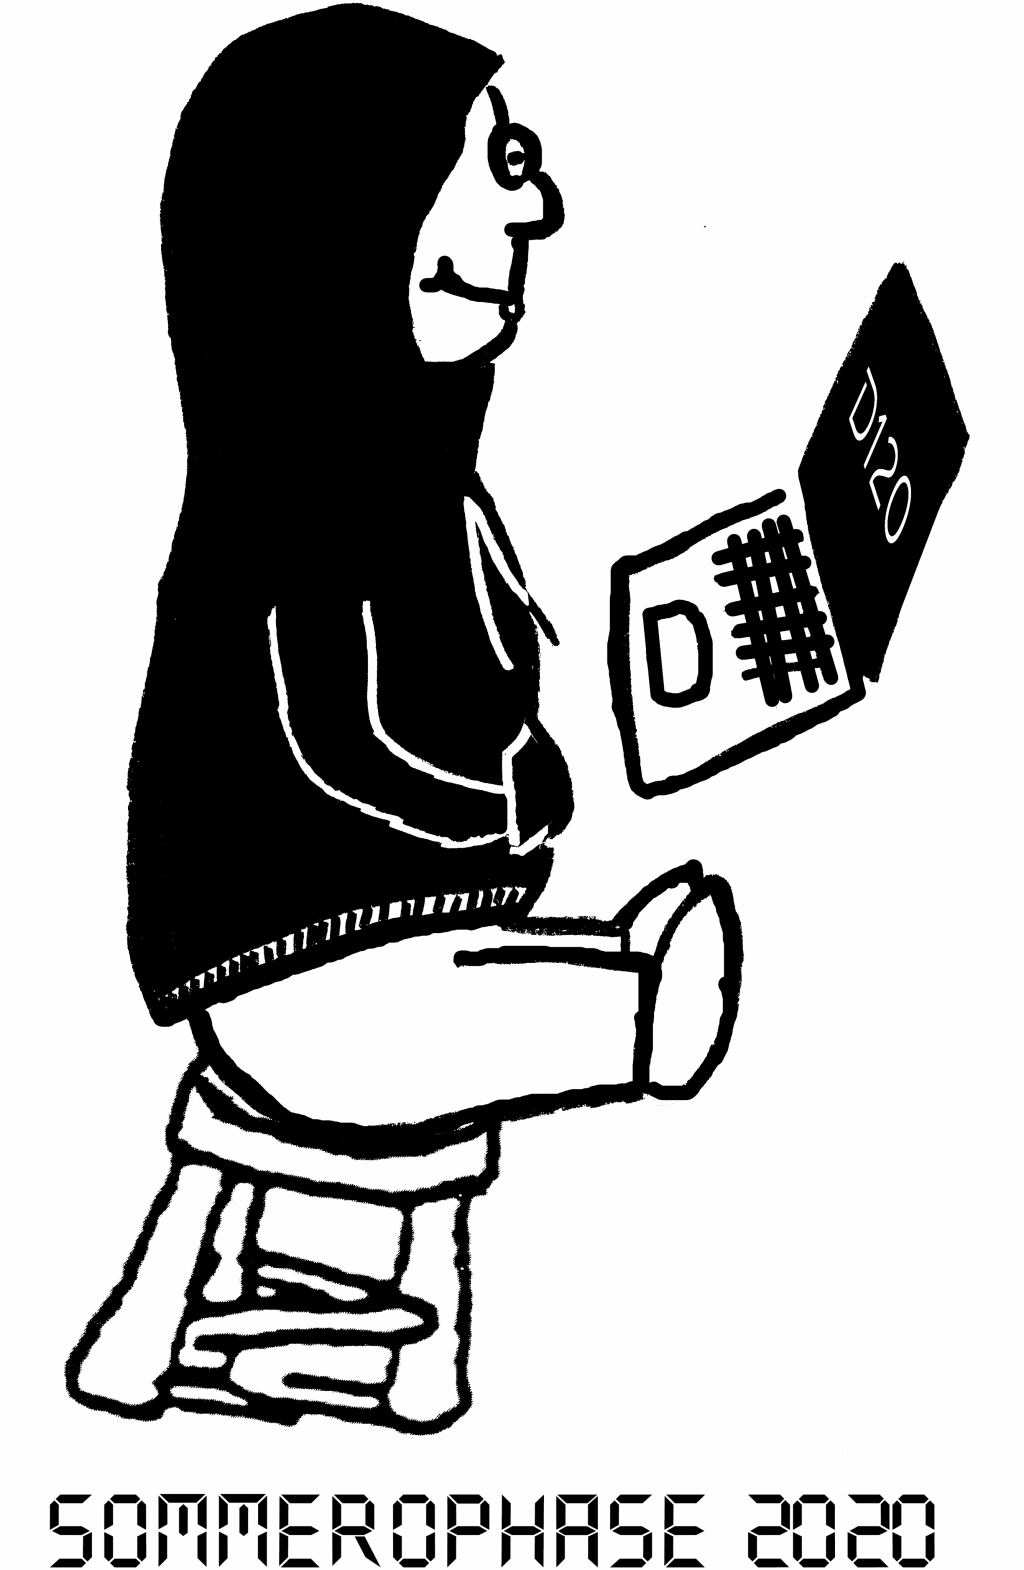
\includegraphics[width=4cm]{../grafik/wesen/wesen_ophase}
\end{textblock*}


\end{document}
